%!TEX root = IntroArithGrps.tex

\mychapter{Basic Properties of Lattices}
\label{BasicLatticesChap}

\prereqs{none.}

This book is about lattices in semisimple Lie groups (with emphasis
on the ``arithmetic'' ones).

\bigskip

\setcounter{equation}{-1} % standing assumps will be numbered 3.0

%% emphasize this! (box with gray border is used here @@@)
\definecolor{grayborder}{gray}{0.6}
\definecolor{whitebkgnd}{gray}{1}
\newlength{\grayborder} \grayborder=10pt \relax 
\newlength{\graygap} \graygap=9pt \relax 
\newlength{\assumpw} \assumpw=\textwidth
	\advance\assumpw -2\grayborder\relax 
	\advance\assumpw -2\graygap\relax
\newbox\assumpbox
\setbox\assumpbox\hbox{\begin{minipage}{\assumpw}%
\begin{standassump} \label{standassump}
Throughout this book:
 \noprelistbreak \parindent=2.2em
 \begin{enumerate}
 \item \label{standassump-G}
 \textbf{\mathversion{bold}$G$ is a linear, semisimple Lie group}
 (see \cref{SSLieGrpDefnSect} for an explanation of these terms),
 with only finitely many connected components,
 and
 \item \label{standassump-Gamma}
 \textbf{\mathversion{bold}$\Gamma$ is a lattice in~$G$} (see \cref{LatticeDefn}).
 \end{enumerate}
 Similar restrictions apply to the symbols $G_1$, $G_2$,
$G'$, $\Gamma_1$, $\Gamma_2$, $\Gamma'$, etc.
\end{standassump}
\end{minipage}%
}
\newlength{\grayh} \grayh=\ht\assumpbox \advance\grayh\dp\assumpbox
	\advance\grayh2\grayborder\relax \advance\grayh2\graygap\relax
\vbox{
\vbox to 0pt{\hbox to \textwidth{\hss\color{grayborder}\vrule width \textwidth height \grayh \hss}\vss}%
\vskip-\baselineskip
\newlength{\whitew} \whitew=\assumpw \advance\whitew2\graygap\relax
\newlength{\whiteh} \whiteh=\grayh \advance\whiteh-2\grayborder\relax
\vbox to 0pt{\vskip\grayborder\hbox to \textwidth{\hss\color{whitebkgnd}\vrule width \whitew height \whiteh \hss}\vss}
\vskip \grayborder \vskip \graygap \vskip-1pt % @@@
\centerline{\copy\assumpbox}
\vskip \grayborder \vskip \graygap
}

\begin{rem}
Without losing any of the main ideas, it may be assumed,
throughout, that $G$ is either $\SL(n,\real)$ or
$\SO(m,n)$ (or a product of these groups), 
%. Much of the material is of interest even in the special case $G = \SO(1,n)$, 
but it is best if the reader is also acquainted with the other
``classical groups\zz,'' such as unitary groups and symplectic groups \csee{ClassicalDefn}. 
\end{rem}

Three definitions in this \lcnamecref{BasicLatticesChap} are very important: lattice subgroups
\pref{LatticeDefn}, commensurable subgroups
\pref{CommensDefn}, and irreducible lattices
(\ref{irreducibleLattice} and~\ref{prodirredlatt}). The
rest of the material in this chapter may not be essential
for a first reading, and can be referred back to when
necessary. However, if the reader has no prior experience
with lattices, then the basic properties discussed
in~\cref{LattDefnSect} will probably be helpful.



\section{Definition} \label{LattDefnSect}

\begin{lem} \label{ExistsFundDom}
  If $\Lambda$ is a discrete subgroup of~$G$, then 
there is a {\normalfont\defit[fundamental!domain!strict]{strict fundamental domain}} for $G/\Lambda$ in~$G$.
That is, there is a Borel subset~$\fund$ of~$G$, such that
the natural map $\fund \to G/\Lambda$, defined
by $g \mapsto g \Lambda$, is bijective.
 \end{lem}

\begin{proof}
 Since $\Lambda$ is discrete, there is a nonempty, open
subset~$U$ of~$G$, such that $(U^{-1} \, U) \cap \Lambda =
\{e\}$. Since $G$ is second countable (or, if you prefer,
since $G$ is $\sigma$-compact), there is a sequence
$\{g_n\}$ of elements of~$G$, such that $\bigcup_{n=1}^\infty g_n
U = G$. Let
 $$ \fund = \bigcup_{n = 1}^\infty \left( 
 \raise1pt\hbox{$\displaystyle % eliminate some blank space % @@@
 g_n U 
\smallsetminus \bigcup_{i< n} g_{i} U \Lambda
$}
  \right) .$$
 Then $\fund$ is obviously Borel, and it is a strict fundamental domain for $G/\Lambda$ 
 \csee{FisFundDom}.
 \end{proof}

\begin{rem} \ 
\noprelistbreak
\begin{enumerate}
\item The above \lcnamecref{ExistsFundDom} is stated for the space $G/\Lambda$ of left cosets of~$\Lambda$, but, in some situations, it is more natural to work with the space $\Lambda \backslash G$ of right cosets. In this book, we will feel free to use whichever is most convenient at a particular time, and leave it to the reader to translate between the two, by using the fact that the function $g \Lambda \mapsto \Lambda g^{-1}$ is a homeomorphism from $G/\Lambda$ to $\Lambda \backslash G$ \csee{LeftCosetsToRightCosets,FundDomRightCosets}. Our choice will usually be determined by the preference for most mathematicians to write their actions on the left. (Therefore, if $G$ is acting, then we will tend to use $G/\Lambda$, but if we are thinking of~$\Lambda$ as acting on~$G$, then we usually consider the quotient $\Lambda \backslash G$.)

\item Definitions in the literature vary somewhat, but saying that a subset~$\fund$ of~$G$ is a \defit[fundamental!domain]{fundamental domain} for $G/\Lambda$ typically means:
	\begin{enumerate}
	\item $\fund \Lambda = G$,
	\item $\fund$ is a closed set that is nice: its interior $\interior\fund$ is dense in~$\fund$, and its boundary $\fund \smallsetminus \interior\fund$ has measure~$0$,
	and
	\item $\fund \lambda \cap \interior\fund = \emptyset$, for all nonidentity $\lambda \in \Lambda$.
	\end{enumerate}
It is not difficult to see that if $\fund$ is a fundamental domain, then it has a Borel subset $\fund'$, such that $\fund'$ is a strict fundamental domain and $\fund \smallsetminus \fund'$ has measure~$0$. This means that, for many purposes (such as calculating integrals), it suffices to have a fundamental domain, rather than finding a set that is precisely a strict fundamental domain.
\end{enumerate}
\end{rem}

\begin{prop} \label{HaarOnHomog}
 Let $\Lambda$ be a discrete subgroup of~$G$, and let
$\mu$ be Haar measure on~$G$. There is a unique
\textup(up to a scalar multiple\textup)
$\sigma$-finite, $G$-invariant Borel measure~$\nu$ on
$G/\Lambda$.
More precisely:
 \begin{enumerate}
 \item \label{HaarOnHomog-nu}
 For any strict fundamental domain~$\fund$, the
measure~$\nu$ can be defined by 
  \begin{equation} \label{HomogFromHaar}
 \nu(A/\Lambda) = \mu( A \cap \fund) ,
 \end{equation}
 for every Borel set~$A$ in~$G$, such that $A \Lambda = A$.
 \item \label{HaarOnHomog-mu}
 Conversely, for $A \subseteq G$, we have
 \begin{equation} \label{HaarFromHomog}
 \mu(A) = \int_{G/\Lambda} \#(A \cap x \Lambda)
\, d \nu(x \Lambda) .
 \end{equation}
 \end{enumerate}
 \end{prop}

\begin{proof} 
 See \cref{HaarOnHomogIsGinv,HaarOnHomog->Haar} for \pref{HaarOnHomog-nu}
and~\pref{HaarOnHomog-mu}. The uniqueness of~$\nu$ follows
from~\pref{HaarOnHomog-mu} and the uniqueness of the Haar
measure~$\mu$.
 \end{proof}

\begin{rem}
 We always assume that the $G$-invariant measure~$\nu$ on
$G/\Lambda$ is normalized so that
\pref{HomogFromHaar} and~\pref{HaarFromHomog} hold.
 \end{rem}

\begin{cor} \label{inject->samemeas}
 Let $\Lambda$ be a discrete subgroup of~$G$, and let
$\phi \colon G \to G/\Lambda$ be the natural
quotient map $\phi(g) = g \Lambda$. If $A$ is a Borel
subset of~$G$, such that the restriction $\phi|_A$ is
injective, then $\nu \bigl( \phi(A) \bigr) = \mu(A)$.
 \end{cor}

\begin{rems} \ \label{VolOnG/Gamma}
 \noprelistbreak
 \begin{enumerate}
 \item \label{VolOnG/Gamma-smooth}
 The Haar measure~$\mu$ on~$G$ is given by a smooth
volume form, so the associated measure~$\nu$ on $G/\Lambda$ is also given by a volume form. Therefore, we say
that $G/\Lambda$ has \defit[finite volume
(homogeneous space)]{finite volume} if $\nu(G/\Lambda) < \infty$.
 \item The assumption that $\Lambda$ is discrete cannot be
eliminated from \cref{HaarOnHomog}. However, a $G$-invariant measure on $G/\Lambda$ can be constructed under the weaker assumption that $\Lambda$ is closed and
unimodular \csee{HaarOnHomog<>unimod}. 
%However, \pref{HomogFromHaar} and \pref{HaarFromHomog} are not valid in this generality.
 \end{enumerate}
 \end{rems}

\begin{defn} \label{LatticeDefn}
 A subgroup~$\Gamma$ of~$G$ is a
\defit[lattice!subgroup]{lattice} in~$G$ if
 \begin{itemize}
 \item $\Gamma$ is a discrete subgroup of~$G$, and
 \item $G/\Gamma$ has finite volume.
 \end{itemize}
 \end{defn}

\begin{rem}
The definition is not vacuous: we will explain in \cref{GHasLatt} that $G$~does have at least one lattice (in fact, infinitely many), although part of the proof will be postponed to \cref{SLnZLattChap}.
\end{rem}

\begin{prop} \label{Latt<>fund}
 Let $\Lambda$ be a discrete subgroup of~$G$, and let
$\mu$ be Haar measure on~$G$. The following are equivalent:
 \begin{enumerate}
 \item \label{Latt<>fund-latt}
 $\Lambda$ is a lattice in~$G$.
 \item \label{Latt<>fund-fund}
 There is a strict fundamental domain~$\fund$ for $G/\Lambda$, with $\mu(\fund) < \infty$.
 \item \label{Latt<>fund-otherside}
 There is a strict fundamental domain~$\fund'$ for $\Lambda \backslash G$, with $\mu(\fund') < \infty$.
 \item \label{Latt<>fund-coarse}
 There is a Borel subset $C$ of~$G$, such that $C \Lambda = G$ and $\mu(C) < \infty$.
 \end{enumerate}
 \end{prop}

\begin{proof}
 ($\ref{Latt<>fund-latt} \Leftrightarrow
\ref{Latt<>fund-fund}$) From \cref{HomogFromHaar}, we
have $\nu(G/\Lambda) = \mu(\fund)$. Therefore,
$G/\Lambda$ has finite volume if and only if
$\mu(\fund) < \infty$.

($\ref{Latt<>fund-fund} \Leftrightarrow \ref{Latt<>fund-otherside}$)
If $\fund$ is any strict fundamental domain for $G/\Lambda$, then $\fund^{-1}$ is a strict fundamental domain for $\Lambda \backslash G$ \csee{FundDomRightCosets}. 
Since $G$ is unimodular, we have $\mu(\fund^{-1}) = \mu(\fund)$ \csee{mu(inverse)}. 

 ($\ref{Latt<>fund-fund} \Rightarrow
\ref{Latt<>fund-coarse}$) Obvious.

 ($\ref{Latt<>fund-coarse} \Rightarrow
\ref{Latt<>fund-latt}$) We have $C \cap x \Lambda \neq
\emptyset$, for every $x \in G$, so, from
\pref{HaarFromHomog}, we see that
 \begin{align*} \nu(G/\Lambda) 
 = \int_{G/\Lambda} 1 \, d\nu(x \Lambda)
 \le \int_{G/\Lambda} \#(C \cap x \Lambda) \,
d\nu(\Lambda x)
 = \mu(C)
 < \infty 
 . & \qedhere \end{align*}
 \end{proof}

\begin{eg}
 As mentioned in \cref{SL2Zlatt}, $\SL(2,\integer)$ is
a lattice in $\SL(2,\real)$.
 \end{eg}

\begin{defn}
 A closed subgroup~$\Lambda$ of~$G$ is
\defit[cocompact subgroup]{cocompact} (or
\defit[uniform subgroup]{uniform}) if $G/\Lambda$ is compact.
 \end{defn}

\begin{cor} \label{Latt<>cpct/finind} \ 
 \noprelistbreak
 \begin{enumerate}
 \item \label{Latt<>cpct/finind-cpct}
 Every cocompact, discrete subgroup of~$G$ is a lattice.
 \item \label{Latt<>cpct/finind-finind}
 Every finite-index subgroup of a lattice is a lattice.
 \end{enumerate}
 \end{cor}

\begin{proof}
 \Cref{cocpct->latt,finindLatt->latt}.
 \end{proof}

\begin{rem}
 Lattices in~$G$ are our main interest, but we will
occasionally encounter lattices in Lie groups~$H$ that
are not semisimple. If $H$ is unimodular, then all of the
above results remain valid with $H$ in the place of~$G$.
In contrast, if $H$ is not unimodular, then
\cref{HaarOnHomog} may fail: there may exist a discrete subgroup~$\Lambda$, such that there is no
$H$-invariant Borel measure on $H/\Lambda$.
Instead, there is sometimes only a semi-invariant
measure~$\nu$:
 $$ \nu(hA) = \Delta(h) \, \nu(A) ,$$
 where $\Delta$~is the modular function of~$H$
\csee{SemiinvariantMeasure}. 
%This is sufficient to
%determine whether $H/\Lambda$ has finite volume
%or not, so \cref{LatticeDefn} applies.
 \end{rem}

For completeness, let us specifically state the following
concrete generalization of \cref{LatticeDefn}
\cf{Latt<>fund}.

\begin{defn} \label{LatticeGeneralDefn}
 A subgroup~$\Lambda$ of a Lie group~$H$ is a
\defit[lattice!subgroup]{lattice} in~$H$ if
 \begin{itemize}
 \item $\Lambda$ is a discrete subgroup of~$H$, and
 \item there is an $H$-invariant measure~$\nu$ on $H/\Lambda$, such that $\nu(H/\Lambda) < \infty$.
% a Borel subset $C$ of~$H$, such that
%$\Lambda C = H$ and $\mu(C) < \infty$, where $\mu$~is the
%left Haar measure on~$H$.
 \end{itemize}
 \end{defn}

\begin{eg}
 $\integer^n$ is a cocompact lattice in~$\real^n$. 
 \end{eg}

\begin{prop}
 If a Lie group~$H$ has a lattice, then $H$~is unimodular.
 \end{prop}

\begin{proof}
 Let $\fund$ be a strict fundamental domain for $H/\Lambda$.
 The proof of \cref{HaarOnHomog} shows $\nu(A/\Lambda) = \nu(A \cap \fund)$, for every Borel set~$A$ in~$G$, such that $A \Lambda = A$. Then \cref{SemiinvariantMeasure} implies $\nu(hA/\Lambda) = \Delta(h) \, \nu(A/\Lambda)$. In particular, we see that $\nu(H/\Lambda) = \Delta(h) \, \nu(H/\Lambda)$, by letting $A = H$  (and noting that $hH = H$).
Since $\nu(H/\Lambda) < \infty$, this implies $\Delta(h) = 1$, as desired.
 \end{proof}

\begin{exercises}[Recall that (in accordance with the Standing Assumptions \pref{standassump}), $\Gamma$~is a lattice in~$G$, and $G$~is a semisimple Lie group.]

\item Show that $\Gamma$ is finite if and only if $G$~is
compact.

\item \label{FisFundDom}
 Complete the proof of \cref{ExistsFundDom}; that
is, show that $\fund$ is a strict fundamental domain.

\item \label{LeftCosetsToRightCosets}
Define $f \colon G/\Lambda \to \Lambda \backslash G$ by $f(g \Lambda) = \Lambda g^{-1}$. Show that $f$ is a homeomorphism.

\item \label{FundDomRightCosets}
Show \cref{ExistsFundDom} easily implies an analogous statement that applies to right cosets. More precisely, show that if 
	\begin{itemize}
	\item $\Lambda$ is a discrete subgroup of~$G$, 
	\item $\fund$ is a strict fundamental domain for $G/\Lambda$, 
	and
	\item $\fund^{-1} = \{\, x^{-1} \mid x \in \fund \,\}$,
	\end{itemize}
then the natural map $\fund^{-1} \to \Lambda \backslash G$, defined
by $g \mapsto \Lambda g$, is bijective.

\item \label{mu(inverse)}
Show that $\mu(A^{-1}) = \mu(A)$ for every Borel subset~$A$ of~$G$.
\hint{Defining $\mu'(A) = \mu(A^{-1})$ yields a $G$-invariant measure on~$G$. The uniqueness of Haar measure implies $\mu' = \mu$. Where did you use the fact that $G$ is unimodular?}

\item \label{mu(fund)}
Let 
\noprelistbreak
	\begin{itemize}
	\item $\Lambda$ be a discrete subgroup of~$G$,
	\item $\fund$ and~$\fund'$ be strict fundamental domains for $G/\Lambda$,
	\item $\mu$ be Haar measure on~$G$,
	and
	\item $A$ be a Borel subset of~$G$.
	\end{itemize}
Show:
	 \begin{enumerate}
	 \item For each $g \in G$, there is a unique $\lambda \in \Lambda$, such that $g \lambda \in \fund$.
	 \item For each $\lambda \in \Lambda$, if we let
	 	 $A_\lambda = \{\, a \in A \mid a \lambda \in \fund \,\}$, then $A_\lambda$ is Borel, and $A$~is the disjoint union of the sets $\{\, A_\lambda \mid
	\lambda \in \Lambda \,\}$.
	 \item $\mu(\fund) = \mu(\fund')$.
	 \item \label{mu(fund)-F=F'}
	 If $A \Lambda = A$, then $\mu(A \cap \fund) = \mu(A \cap
	\fund')$.
	 \end{enumerate}

\item \label{HaarOnHomogIsGinv}
 Show, for every Haar measure~$\mu$ on~$G$, that the Borel
measure~$\nu$ defined in \fullcref{HaarOnHomog}{nu} is
$G$-invariant.
 \hint{For any $g \in G$, the set $g \fund$ is a strict
fundamental domain. From \fullcref{mu(fund)}{F=F'}, we
know that $\nu$~is independent of the choice of the strict
fundamental domain~$\fund$.}

\item \label{HaarOnHomog->Haar}
 If $\Lambda$ is a discrete subgroup
of~$G$, and $\nu$ is a $\sigma$-finite, $G$-invariant
Borel measure on $G/\Lambda$, show that the Borel
measure~$\mu$ defined in \fullcref{HaarOnHomog}{mu} is
$G$-invariant.

\item \label{HaarOnHomog<>unimod}
 Let $H$ be a closed subgroup of~$G$. Show that there is a
$\sigma$-finite, $G$-invariant Borel measure~$\nu$ on
$G/H$ if and only if $H$~is unimodular.
 \hint{($\Rightarrow$) For a left Haar measure~$\rho$
on~$H$, define a left Haar measure~$\mu$ on~$G$ by
 $$ \mu(A) = \int_{G/H} \rho(x^{-1} A \cap H) \,
d \nu(xH) .$$
 Then $\mu(A) = \Delta_H(h) \, \mu(Ah)$ for $h \in H$,
where $\Delta_H$ is the \term{modular function} of~$H$. Since
$G$ is unimodular, we must have $\Delta_H \equiv 1$.}

\item \label{finext->latt}
 Show that if $\Lambda$ is a discrete subgroup of~$G$
that contains~$\Gamma$, then $\Lambda$ is a lattice
in~$G$, and $\Gamma$ has finite index in~$\Lambda$.
\hint{Let $\fund$ be a strict fundamental domain for $G/\Lambda$, and let $F$~be a set of coset representatives for $\Gamma$ in~$\Lambda$. Then $\fund \cdot F$ is a strict fundamental domain for $G/\Gamma$, and therefore has finite measure.}

\item \label{CpctInHomog}
 Let $\Lambda$ be a discrete subgroup of~$G$. Show
that a subset~$A$ of $G/\Lambda$ is precompact
if and only if there is a compact subset~$C$ of~$G$, such
that $A \subseteq C\Lambda / \Lambda$.
 \hint{($\Leftarrow$) The continuous image of a compact
set is compact. ($\Rightarrow$) Let $\mathcal{U}$ be a
cover of~$G$ by precompact, open sets.} 

\item \label{cocpct->latt}
 Prove \fullcref{Latt<>cpct/finind}{cpct}.
 \hint{\cref{CpctInHomog} and
\fullcref{Latt<>fund}{coarse}.}

\item \label{finindLatt->latt}
 Prove \fullcref{Latt<>cpct/finind}{finind}.
 \hint{\cref{Latt<>fund}. A finite union of sets
of finite measure has finite measure.}

\item \label{SemiinvariantMeasure}
 Let 
 \begin{itemize}
 \item $H$ be a Lie group,
 \item $\Lambda$ be a discrete subgroup of~$H$,
 \item $\mu$ be the right Haar measure on~$H$,
 and
 \item $\fund$ be a strict fundamental domain for $H/\Lambda$. %such that $\mu(\fund) < \infty$.
 \end{itemize}
 Define a $\sigma$ Borel measure~$\nu$ on $H/\Lambda$ by 
 $ \nu(A/\Lambda) = \mu( A \cap \fund) $,
 for every Borel set~$A$ in~$H$, such that $A \Lambda =
A$. Show $\nu(h A / \Lambda) =
\Delta(h) \, \nu(A/\Lambda)$, where $\Delta$~is
the modular function of~$H$.
 \hint{Cf.\ \cref{HaarOnHomogIsGinv}.}

%\item Suppose $\Gamma_1$ and~$\Gamma_2$ are lattices
%in~$G$, such that $\Gamma_1 \subseteq \Gamma_2$. Show that
%$\Gamma_1$ has finite index in~$\Gamma_2$.

\item Show that every discrete, cocompact subgroup of every Lie group is a lattice.
\hint{Define $\nu$ as in \cref{SemiinvariantMeasure}. Since %$H/\Lambda$ is compact, we know 
$\nu(H/\Lambda)< \infty$ (why?), we must have $\Delta(h) = 1$.}

\end{exercises}





\section{Commensurability and isogeny} \label{CommSect}

We usually wish
to ignore the minor differences that come from passing to a finite-index
subgroup. The following
definition describes the resulting equivalence relation.

\begin{defn} \label{CommensDefn}
 We say that two subgroups~$\Lambda_1$ and~$\Lambda_2$ of a group~$H$ are
\defit{commensurable} if $\Lambda_1 \cap \Lambda_2$ is a
finite-index subgroup of both~$\Lambda_1$ and~$\Lambda_2$.
This is an equivalence relation on the collection of all
subgroups of~$H$ \csee{CommEquiv}.
 \end{defn}

\begin{egs} \ \label{CommensEg}
\noprelistbreak
 \begin{enumerate}
 \item Two cyclic subgroups $a \integer$
and~$b \integer$ of~$\real$ are commensurable if and
only if $a$ is a nonzero rational multiple of~$b$; therefore,
commensurability of subgroups generalizes the classical
notion of commensurability of real numbers.

 \item \label{CommensEg-latt}
 It is easy to show that every subgroup commensurable
to a lattice is itself a lattice. (For example, this follows from
\fullcref{Latt<>cpct/finind}{finind} and
\cref{finext->latt}.)
 \end{enumerate}
 \end{egs}

The analogous notion for Lie groups (with finite center and finitely many connected components) is called ``isogeny:''

\begin{defns} \  \label{IsogenyDefn}
\noprelistbreak
	\begin{enumerate}
	\item $G_1$ is \defit{isogenous} to~$G_2$ if some finite cover of~$(G_1)^\circ$ is isomorphic to some finite cover of~$(G_2)^\circ$. This is an equivalence relation.
	\item A (continuous) homomorphism $\varphi \colon G_1 \to G_2$ is an \defit{isogeny} if it is an isomorphism modulo finite groups. More precisely:
	\begin{itemize}
	\item the kernel of~$\varphi$ is finite,
	and
	\item the image of~$\varphi$ has finite index in~$G_2$.
	\end{itemize}
	\end{enumerate}
\end{defns}

\begin{rem}
The following are equivalent:
	\begin{enumerate}
	\item $G_1$ is isogenous to~$G_2$.
	\item $\Ad (G_1)^\circ \iso \Ad (G_2)^\circ$.
	\item $G_1$ and~$G_2$ are \defit[locally!isomorphic]{locally isomorphic}, that is, the Lie
algebras $\Lie G_1$ and~$\Lie G_2$ are isomorphic.
	\item There is an isogeny from some finite cover of~$(G_1)^\circ$ to~$G_2$.
	\end{enumerate}
\end{rem}

The normalizer of a subgroup is very important in group
theory. Because we are ignoring finite groups, the
following definition is natural in our context.

\begin{defn}
 An element~$g$ of~$G$ \emph{commensurates}~$\Gamma$ if
$g \Gamma g^{-1}$ is commensurable to~$\Gamma$. Let
 $$\Comm_G(\Gamma) = \{\, g \in G \mid \text{$g$
commensurates~$\Gamma$} \,\} .$$
 This is called the \defit{commensurator} of~$\Gamma$.
 %(or the \defit{commensurability subgroup} of~$\Gamma$).
 \end{defn}

\begin{rem}
 The commensurator of~$\Gamma$ is sometimes much larger than the
normalizer of~$\Gamma$. For example, let $G =
\SL(n,\real)$ and $\Gamma = \SL(n,\integer)$. Then
$\nzer_G(\Gamma)$ is commensurable to~$\Gamma$
\csee{latticenormalizer}, but $\Comm_G(\Gamma)$ contains $\SL(n,\rational)\mk$\csee{SLQCommSLZ}, so $\Comm_G(\Gamma)$
is dense in~$G$, even though $\nzer_G(\Gamma)$ is discrete.
Therefore, in this example (and, more generally, whenever
$\Gamma$ is ``arithmetic''), $\nzer_G(\Gamma)$ has infinite
index in $\Comm_G(\Gamma)$.

On the other hand, if $G = \SO(1,n)$, then it is known
that there are examples in which $\Gamma$, $\nzer_G(\Gamma)$,
and $\Comm_G(\Gamma)$ are commensurable to each other
(see \cref{Comm(Gamma)discrete}
and \cref{NonarithInSO1n}).
 \end{rem}

\begin{defn}
 We say that two groups $\Lambda_1$ and~$\Lambda_2$ are
\defit[commensurable!abstractly]{abstractly commensurable} if some finite-index subgroup of~$\Lambda_1$ is isomorphic to some finite-index subgroup
of~$\Lambda_2$.
 \end{defn}

Note that if $\Lambda_1$ and~$\Lambda_2$ are
commensurable, then they are abstractly commensurable, but not
conversely.

\begin{exercises}

\item \label{CommEquiv}
 Verify that commensurability is an equivalence relation.

\item If $\Gamma_1$ is commensurable
to~$\Gamma_2$, show $\Comm_G(\Gamma_1) =
\Comm_G(\Gamma_2)$.

\end{exercises}





\section{Irreducible lattices} \label{IrredLattSect}

Note that $\Gamma_1 \times \Gamma_2$ is a lattice in $G_1
\times G_2$. A lattice that can be decomposed as a product
of this type is said to be \defit[reducible!lattice]{reducible}.

\begin{defn} \label{irreducibleLattice}
 $\Gamma$ is \defit[irreducible!lattice]{irreducible} if $\Gamma N$ is dense
in~$G$, for every noncompact, closed, normal subgroup~$N$
of~$G^\circ$ (and $\Gamma$ is infinite, or, equivalently, $G$~is not compact).
 \end{defn}

\begin{eg}
If $G$ is simple (and not compact), then
every lattice in~$G$ is irreducible.  Conversely, if $G$
is not simple, then not every lattice
in~$G$ is irreducible.  To see this, assume, for
simplicity, that $G$ is connected and has trivial center (and is not compact). Then we may write
$G$ as a nontrivial direct product $G = G_1 \times G_2$,
where each of $G_1$ and~$G_2$ is semisimple. If we let
$\Gamma_i$ be any lattice in~$G_i$, for $i = 1,2$, then
$\Gamma_1 \times \Gamma_2$ is a reducible lattice in~$G$.
\end{eg}

The following \lcnamecref{prodirredlatt} shows (under mild assumptions)
that every lattice is commensurable to a product of irreducible
lattices. Therefore, the preceding example provides essentially
the only way to construct reducible lattices, so most
questions about lattices can be reduced to the irreducible
case. We postpone the proof, because
it relies on some results from later in this \lcnamecref{BasicLatticesChap}.

\begin{prop}[(see proof on \cpageref{prodirredlattPf})] \label{prodirredlatt}
 Assume 
 \noprelistbreak
 \begin{itemize}
 \item $G$ has trivial center,
  and 
 \item $\Gamma$ projects densely into the maximal compact
factor of~$G$. 
 \end{itemize}
 Then there is a direct-product decomposition $G = G_1 \times
\cdots \times G_r$, such that $\Gamma$ is commensurable
to\/ $\Gamma_1 \times \cdots \times \Gamma_r$, where\/
$\Gamma_i = \Gamma \cap G_i$, and\/ $\Gamma_i$ is an
irreducible lattice in~$G_i$, for each~$i$.
 \end{prop}

For readers familiar with locally symmetric spaces, these results can be restated in the following geometric
terms. 

\begin{defn}
 Recall that a locally symmetric space $\Gamma \backslash
X$ is \defit[irreducible!locally symmetric space]{irreducible} if there do not exist (nontrivial)
locally symmetric spaces $\Gamma_1 \backslash X_1$ and
$\Gamma_2 \backslash X_2$, such that the product
 $ (\Gamma_1 \backslash X_1) \times (\Gamma_2 \backslash
X_2)$
 finitely covers $\Gamma \backslash X$.
 \end{defn}

The following is obvious by induction on $\dim X$.

\begin{prop}
 There exist locally symmetric spaces\/
 $\Gamma_1 \backslash X_1, \ldots, \Gamma_r \backslash X_r$
 that are irreducible, such
that the product\/
 $ (\Gamma_1 \backslash X_1) \times \cdots \times (\Gamma_r
\backslash X_r)$
 finitely covers $\Gamma \backslash X$.
 \end{prop}

The following is a restatement of
\cref{prodirredlatt} (in the special case where $G$
has no compact factors).

\begin{prop} 
 Let $M$ be an irreducible locally symmetric space, such
that the universal cover~$X$ of~$M$ has no compact
factors, and no flat factors. For any nontrivial cartesian
product decomposition $X = X_1 \times X_2$ of~$X$, the
image of~$X_1$ is dense in~$M$.
 \end{prop}

We will see in \cref{SL(2Z[sqrt2])} that
$\SL(2,\real) \times \SL(2,\real)$ has an irreducible
lattice (for example, a lattice isomorphic to
$\SL\bigl( 2,\integer[\sqrt{2}] \bigr)$). 
More generally, \cref{Isotypic->irred} shows
that $G$ has an irreducible lattice if all the simple factors of the ``\term{complexification}'' of~$G$ are isogenous to each other. The converse is proved in \cref{irred->isotypic}, under the additional assumption that $G$ has no compact factors.

\begin{exercises}

\item \label{irred->CpctFactor}
 Show that if $\Gamma$ is irreducible, %and $G$~is not compact, 
then $\Gamma$ projects densely into the maximal
compact factor of~$G$.

\end{exercises}



\section{\texorpdfstring{Unbounded subsets of $\Gamma \backslash G$}{Unbounded subsets of G/Γ}} % should be Γ\G, but that gives a TeX error @@@
\label{DivergeSect}

 Geometrically, looking at the fundamental
domain described in \cref{SL2Zlatt} makes it clear that the sequence
$\{ni\}$ tends to~$\infty$ in $\SL(2,\integer) \backslash
\hyperbolic^2$. In this section, we give an algebraic
criterion that determines whether or not a sequence tends
to~$\infty$ in $G/\Gamma$, without any need for
a fundamental domain.

Recall that the \defit{injectivity radius} of a Riemannian
manifold~$X$ is the maximal $r \ge 0$, such that, for
every $x \in X$, the exponential map is a diffeomorphism
on the open ball of radius~$r$ around~$x$. If $X$~is
compact, then the injectivity radius is nonzero. The
following proposition shows that the converse holds in the
special case where $X = \Gamma \backslash G/K$ is locally
symmetric of finite volume.

\begin{prop} \label{Cpct<>InjRad}
 For $g \in G$, define $\phi_g \colon G \to G/\Gamma$ by 
 $\phi_g(x) = xg\Gamma$. The homogeneous
space $G/\Gamma$ is compact if and only if
there is a nonempty, open subset~$U$ of~$G$, such that,
for every $g \in G$, the restriction $\phi_g|_U$
of~$\phi_g$ to~$U$ is injective.
 \end{prop}

\begin{proof}
 ($\Rightarrow$) Define $\phi \colon G \to G/\Gamma$ 
 by $\phi(x) = x \Gamma$. Then $\phi$~is a
covering map, so, for each $p \in G/\Gamma$,
there is a connected neighborhood~$V_p$ of~$p$, such that
the restriction of~$\phi$ to each component of
$\phi^{-1}(V_p)$ is a diffeomorphism onto~$V_p$. Since
$\{\, V_p \mid p \in G/\Gamma\}$ is an open
cover of $G/\Gamma$, and $G/\Gamma$
is compact, there is a connected neighborhood~$U$ of~$e$
in~$G$, such that, for each $p \in G/\Gamma$,
there is some $p' \in G/\Gamma$, with $Up
\subseteq V_{p'}$ \csee{LebesgueNumberG}. Then $\phi_g|_U$
is injective, for each $g \in G$.

($\Leftarrow$) We prove the contrapositive. Let $U$ be any
nonempty, precompact, open subset of~$G$. (We wish to show,
for some $g \in G$, that $\phi_g|_U$ is not injective.)
 If $C$ is any compact subset of $G/\Gamma$,
then, because $G/\Gamma$ is not compact, we
have 
 $$ (G/\Gamma) \smallsetminus (U^{-1} C) \neq
\emptyset .$$
 Hence, we may inductively construct a sequence
$\{g_n\}$ of elements of~$G$, such that the open sets
$\phi_{g_1}(U), \phi_{g_2}(U), \ldots$ are pairwise
disjoint. Since $G/\Gamma$ has finite volume,
these sets cannot all have the same volume, so, for
some~$n$, the restriction $\phi_{g_n}|_U$ is not injective
\csee{inject->samemeas}. 
 \end{proof}

Let us restate this geometric result in algebraic terms.

\begin{notation}
 For elements $a$ and~$b$ of a group~$H$, and subsets~$A$
and~$B$ of~$H$, let%
	\nindex{${}^b \! a = b a b^{-1}$ for $a,b \in G$}%
	\nindex{${}^G\Gamma$ = $\{\, {}^g \gamma \mid \gamma \in \Gamma, \ g \in G \,\}$}
\begin{align*}
	{}^b \! a &= b a b^{-1} , 
	&
	{}^B \! a &= \{\, {}^b \!a \mid b \in B\,\}, \\
 	{}^b \! A &= \{\, {}^b \!a \mid a \in A \,\}, 
 	&
	{}^B \! A &= \{\, {}^b \!a \mid a\in A, b \in B \,\}
 	. \end{align*}
  \end{notation}

\begin{cor} \label{G/GammaCpct<>NoAccPt}
 $G/\Gamma$ is compact if and only if the
identity element~$e$ is \textbf{not} an accumulation point
of\/ ${}^G\Gamma$.
 \end{cor}

\begin{proof}
 We have
\begin{align*} 
\text{$\phi_g|_U$ is injective}
 &\quad \Leftrightarrow \quad 
 \nexists u_1,u_2 \in U, \ 
 \text{$u_1 g \Gamma = u_2 g \Gamma$ \  and \ $u_1 \neq u_2$}
 \\&\quad \Leftrightarrow \quad 
 {}^g \Gamma \cap (U^{-1} U) = \{e\} 
 . \qedhere \end{align*}
 \end{proof}

This has the following interesting consequence.

\begin{cor} \label{GammaUnip->notcpct}
 If\/ $\Gamma$ has a nontrivial, \index{unipotent!element}{unipotent element}, then
$G/\Gamma$ is \textbf{not} compact.
 \end{cor}

\begin{proof}
 If $u$~is a nontrivial, unipotent element
of~$\Gamma$, then, from the \thmindex{Jacobson-Morosov}{Jacobson-Morosov Lemma}
\pref{JacobsonMorosov}, we know there is a continuous
homomorphism $\phi \colon \SL(2,\real) \to G$, with 
 $\phi 
 \begin{Smallbmatrix}
 1 & 1 \\
 0 & 1
 \end{Smallbmatrix}
 = u$.  
 Let 
 $ a = \phi 
 \begin{Smallbmatrix}
  1/2 & 0 \\
 0 & 2
 \end{Smallbmatrix}
 \in G $.
 Then
 \goodbreak % @@@
 \begin{align*}
  a^{n} \, u \, a^{-n} 
 &= \phi 
 \left( 
 \begin{bmatrix}
 2^{-n} & 0 \\
 0 & 2^n
 \end{bmatrix}
 \begin{bmatrix}
 1 & 1 \\
 0 & 1
 \end{bmatrix}
 \begin{bmatrix}
 2^n & 0 \\
 0 & 2^{-n}
 \end{bmatrix}
 \right)
 \\&= 
 \phi
 \left( \begin{bmatrix}
 1 & 2^{-2n} \\
 0 & 1
 \end{bmatrix} \right)
 \to
 \phi
 \left( \begin{bmatrix}
 1 & 0 \\
 0 & 1
 \end{bmatrix} \right)
 = e .\end{align*}
 Therefore, $e$~is an accumulation point of ${}^G u$, so
\cref{G/GammaCpct<>NoAccPt} implies that $G/\Gamma$ is not compact.
 \end{proof}

\begin{rems} \  \label{GodementConverse}
\noprelistbreak
	\begin{enumerate}
	\item If $G$ has no compact factors, then the converse of
\cref{GammaUnip->notcpct} is true.
However, we will prove this only in the special case where $\Gamma$ is
``arithmetic'' \csee{GodementSect}.
	\item In general (without any assumption on compact factors), it can be shown that $G/\Gamma$ is compact if and only if every element of~$\Gamma$ is semisimple \csee{CocpctAllSS}.
	\end{enumerate}
\end{rems}

The proofs of \cref{Cpct<>InjRad} and
\cref{G/GammaCpct<>NoAccPt} establish the following
more general version of those results.

\begin{prop}[\csee{diverge<>contractEx}] \label{diverge<>contract}
 Let $\Lambda$ be a lattice in a Lie group~$H$, and let
$C$ be a subset of~$H$. The image of~$C$ in $H/\Lambda$ is 
precompact if and only if the identity
element~$e$ is \textbf{not} an accumulation point of\/
${}^C \! \Lambda$.
 \end{prop}

The following is a similar elementary result that applies
to the important special case where $G = \SL(\ell,\real)$
and $\Gamma = \SL(\ell,\integer)$, without relying on the
fact that $\SL(\ell,\integer)$ is a lattice. 
%For
%convenience, the result discusses $G/\Gamma$, rather than
%$\Gamma \backslash G$ (because we write $gv$, not~$vg$,
%for $g \in G$ and $v \in \real^\ell$). Since $\Gamma
%\backslash G$ is diffeomorphic to $G/\Gamma$ (via the map
%$\Gamma g \mapsto g^{-1} \Gamma$), this change of notation
%is of no real significance.

\begin{prop}[(\thmindex{Mahler Compactness Criterion}Mahler Compactness Criterion)]
\label{MahlerCpct}
 Let $C \subseteq \SL(\ell,\real)$. The image of~$C$ in\/
$\SL(\ell,\real)/\SL(\ell,\integer)$ is precompact if and
only if\/ $0$~is \textbf{not} an accumulation point of 
 $$ C \integer^\ell = \{\, cv \mid c \in C, v \in
\integer^\ell  \,\} .$$
 \end{prop}

\begin{proof}
 ($\Rightarrow$)  Since the image of~$C$ in
$\SL(\ell,\real)/\SL(\ell,\integer)$ is precompact, there
is a compact subset~$C_0$ of~$G$, such that $C \subseteq C_0
\SL(\ell,\integer)$ \csee{CpctInHomog}. There is no harm in
assuming that $C = C_0 \SL(\ell,\integer)$ (by enlarging~$C$). Then
 $ C \bigl( \integer^\ell \smallsetminus \{0\} \bigr) 
 = C_0 \bigl( \integer^\ell \smallsetminus \{0\} \bigr) 
 $
 is closed (since $\integer^\ell \smallsetminus \{0\}$,
being discrete, is closed and $C_0$~is compact), so $C
\bigl( \integer^\ell \smallsetminus \{0\} \bigr)$ contains
all of its accumulation points. In addition, since $0$~is
fixed by every element of~$C$, we know that $0 \notin C
\bigl( \integer^\ell \smallsetminus \{0\} \bigr)$.
Therefore, $0$~is not an accumulation point of $C \bigl(
\integer^\ell \smallsetminus \{0\} \bigr)$.

($\Leftarrow$) To simplify the notation (while retaining
the main ideas), let us assume $\ell = 2$
\csee{MahlerCpctPfExer}. Suppose $\{g_n\}$ is a sequence
of elements of~$\SL(2,\real)$, such that $0$~is
\textbf{not} an accumulation point of $\bigcup_{n=1}^\infty
g_n \integer^2$. We wish to show there is a
sequence $\{\gamma_n\}$ of elements of $\SL(2,\integer)$,
such that $\{g_n \gamma_n\}$ has a convergent subsequence.

For each~$n$, let 
\noprelistbreak
 \begin{itemize}
 \item $v_n \in \integer^2 \smallsetminus \{0\}$, such
that $\|g_n v_n\|$ is minimal,
 \item $\pi_n \colon \real^2 \to \real g_n v_n$ and
 $\pi_n^\perp \colon \real^2 \to (\real g_n v_n)^\perp$
 be the orthogonal projections, and
 \item $w_n \in \integer^2 \smallsetminus \real v_n$, such
that $\| \pi_n^\perp(g_n w_n)\|$ is minimal. 
 \end{itemize}
 By replacing $w_n$ with $w_n + k v_n$, for an appropriately chosen $k \in
\integer$, we may assume $\|\pi_n(g_n w_n)\| \le \|g_n
v_n\|/2$. Then, since the minimality of $\|g_n v_n\|$ implies
$\| g_n v_n \| \le \| g_n w_n \|$, we have 
 $$ \| g_n v_n \|
% \le \| g_n w_n \|
 \le \| \pi_n^\perp(g_n w_n)\| + \|\pi_n(g_n w_n)\|
 \le \| \pi_n^\perp(g_n w_n)\| + \frac{\| g_n v_n \|}{2}
,$$
 so
 \begin{equation} \label{LowerBdOnWn}
 \|\pi_n^\perp(g_n w_n)\| \ge \frac{\| g_n v_n \|}{2} .
 \end{equation}

Let $C$ be the convex hull of $\{0,v_n,w_n\}$ and
(thinking of $v_n$ and~$w_n$ as column vectors) let
$\gamma_n = \bigl[ v_n \  w_n \bigr] \in \Mat_{2\times 2}(\integer)$.
From the minimality of $\|g_n v_n\|$ and $\|
\pi_n^\perp(g_n w_n)\|$, we see that $C \cap \integer^2 =
\{0,v_n,w_n\}$ \csee{min->ConvHull}, so $\det \gamma_n =
\pm 1$ \csee{DetOne}.
Therefore, perhaps after replacing $w_n$ with~$-w_n$, we
have $\gamma_n \in \SL(2,\integer)$. Since 
	$\gamma_n \! \left[ \begin{smallmatrix} 1 \\ 0 \end{smallmatrix} \right] = v_n$ 
and $\gamma_n \! \left[ \begin{smallmatrix} 0 \\ 1 \end{smallmatrix} \right] = w_n$, 
we may assume, by
replacing $g_n$ with~$g_n \gamma_n$, that 
 $$ \mbox{$v_n = \left[ \begin{smallmatrix} 1 \\ 0 \end{smallmatrix} \right]$
 \qquad and\qquad 
 $w_n = \left[ \begin{smallmatrix} 0 \\ 1 \end{smallmatrix} \right]$.} $$

Note that 
 \begin{equation} \label{det=gvxperp}
 \|\pi_n^\perp (g_n w_n)\| \cdot \|g_n v_n \|
 = \det g_n
 = 1 .
 \end{equation}
 By combining this with \pref{LowerBdOnWn}, we see that
$\{ g_n v_n\}$ is a bounded sequence, so, by passing to a
subsequence, we may assume $g_n v_n$ converges to some
vector~$v$. By assumption, we have $v \neq 0$.

Now, from \pref{det=gvxperp}, and the fact that $\|g_n v_n
\| \to \|v\|$ is bounded away from~$0$, we see that
$\|\pi_n^\perp (g_n w_n)\|$ is bounded. Because
$\|\pi_n(g_n w_n)\|$ is also bounded, we conclude that
$\|g_n w_n\|$ is bounded. Hence, by passing to a
subsequence, we may assume $g_n w_n$ converges to some
vector~$w$. From \pref{LowerBdOnWn}, we know that
$\|\pi_n^\perp(g_n w_n)\| \not\to 0$, so $w \notin \real
v$.

Since $v \neq 0$ and $w \notin \real v$, there is some $g
\in \GL(\ell,\real)$ with $g \! \left[ \begin{smallmatrix} 1 \\ 0 \end{smallmatrix} \right] = v$ and $g \! \left[ \begin{smallmatrix} 0 \\ 1 \end{smallmatrix} \right] = w$.
We have 
 $$ g_n \! \left[ \begin{smallmatrix} 1 \\ 0 \end{smallmatrix} \right] = g_n v_n \to v = g \! \left[ \begin{smallmatrix} 1 \\ 0 \end{smallmatrix} \right] $$
 and, similarly, $g_n \!  \left[ \begin{smallmatrix} 0 \\ 1 \end{smallmatrix} \right] \to g \! \left[ \begin{smallmatrix} 0 \\ 1 \end{smallmatrix} \right]$, so $g_n x \to gx$
for all $x \in \real^2$. Therefore, $g_n \to g$, as desired.
 \end{proof}
 
\begin{exercises}

\item \label{LebesgueNumberG}
 Suppose a Lie group~$H$ acts continuously on a compact
topological space~$M$, and $\mathcal{V}$~is an open cover
of~$M$. Show that there is a neighborhood~$U$ of~$e$
in~$H$, such that, for each $m \in M$, there is some $V
\in \mathcal{V}$ with $Um \subseteq V$.
 \hint{This is analogous to the fact that every open cover
of a compact metric space has a ``\term[Lebesgue!number]{Lebesgue number}\zz.''
Each $m \in M$ is contained in some $V_m \in \mathcal{V}$. Choose $V_m'$ containing~$m$, and a neighborhood $U'_m$ of~$e$, such that $U'_m V_m' \subseteq V_m$. Cover $M$ with finitely many $V_m'$.}

\item \label{diverge<>contractEx}
Prove \cref{diverge<>contract}.
\hint{See the proofs of \cref{Cpct<>InjRad} and
\cref{G/GammaCpct<>NoAccPt}.}
% For convenience, let 
% $$ A = (\Lambda \smallsetminus \{e\})^C .$$
%
% ($\Rightarrow$) Since the image of~$C$ in $\Lambda
%\backslash H$ is precompact, there is a compact
%subset~$C_0$ of~$H$, such that $C \subseteq \Lambda C_0$
%\csee{CpctInHomog}. By enlarging~$C$, we may assume that
%$C = \Lambda C_0$. Then
% $$ A
% = \bigl( \Lambda \smallsetminus \{e\} \bigr) ^{\Lambda
%C_0}
% = \bigl( \Lambda \smallsetminus \{e\} \bigr) ^{C_0}
% $$
% is closed (since $\Lambda \smallsetminus \{e\}$, being
%discrete, is closed and $C_0$~is compact), so $A$ contains
%all of its accumulation points. In addition, since $e$ is
%not conjugate to any element of $\Lambda \smallsetminus
%\{e\}$, we know that $e \notin A$. Therefore, $e$~is not
%an accumulation point of~$A$.
%
%($\Leftarrow$) We prove the contrapositive. Let $U$ be any
%precompact, symmetric neighborhood of~$e$ in~$H$. (It
%suffices to show $U^2 \cap A \not= \emptyset$.) Note that
% $$ A = \bigcup_{c \in C} \Stab_H(\Lambda c) \smallsetminus
%\{e\} ,$$
% where, for each $p \in \Lambda \backslash H$, we define
% $$ \Stab_H(p) = \{\, h \in H \mid ph = p \,\} .$$
% If $K$ is any compact subset of~$H$, then, because the
%image of~$C$ in $\Lambda \backslash H$ is not compact, we
%have $C \smallsetminus (\Lambda K U^2) \neq \emptyset$.
%Therefore, by induction on~$n$, we may choose a sequence
%$\{c_n\}$ of elements of~$C$, such that the open sets
%$\Lambda c_1 U, \Lambda c_2 U, \ldots$ are pairwise
%disjoint. Since $\Lambda \backslash H$ has finite volume,
%the images of these sets cannot all have the same volume
%in $\Lambda \backslash H$, so, for some~$n$, the map $U
%\to \Lambda \backslash H \colon u \mapsto \Lambda c_n u$
%is not injective \see{inject->samemeas}. Therefore, there exist
%$u_1$ and~$u_2$ in~$U$, such that $u_1 \neq u_2$, and
%$\Lambda c_n u_1 = \Lambda c_n u_2$. Then
% $$ u_1 u_2^{-1} \in U^2 \cap \Stab_H(\Lambda c_n)
% \subseteq U^2 \cap \bigl( A \cup \{e\} \bigr) ,$$
% and $u_1 u_2^{-1} \neq e$, so $U^2 \cap A \neq
%\emptyset$, as desired.

\item \label{LattInH->ProperMap}
 Use \cref{diverge<>contract} to show that if
$H$ is a closed subgroup of~$G$, such that $H/\Gamma$
is a lattice in~$H$, then the natural inclusion map 
 $H/(\Gamma \cap H) \hookrightarrow G/\Gamma$ is proper.
 \hint{It suffices to show that if $C$ is a subset of~$H$,
such that the image of~$C$ in $G/\Gamma$ is
precompact, then the image of~$C$ in $H/(\Gamma \cap H)$ is also precompact.}

\item Let $G = \SL(2,\real)$, $\Gamma = \SL(2,\integer)$,
and $A$~be the subgroup consisting of all the diagonal
matrices in~$G$. Show that the natural inclusion map 
 $A/(\Gamma \cap A) \hookrightarrow G/\Gamma$ is proper, but $\Gamma \cap A$ is \emph{not}
a lattice in~$A$. (Therefore, the converse of
\cref{LattInH->ProperMap} does not hold.)

\item Let $G = \SL(3,\real)$, $\Lambda = \SL(3,\integer)$, and $a = \diag(1/2, \, 1, \, 2)
% \begin{bmatrix}
% 1/2 & 0 & 0 \\
% 0 & 1 & 0 \\
% 0 & 0 & 2
% \end{bmatrix}
 \in H$.
 Show that $a^n \Lambda \to \infty$ in $G/\Lambda$ 
 as $n \to \infty$. That is, show, for each compact
subset~$C$ of $G/\Lambda$, that, for all
sufficiently large~$n$, we have $a^n \Lambda \notin C$.
(For the purposes of this exercise, do \emph{not} assume
that $\Lambda$ is a lattice in~$G$.)

%\item Show that if $\Gamma$ contains a nontrivial
%unipotent element, then $\Gamma \backslash G$ is not
%compact.

%\item Prove ($\Rightarrow$) of \cref{MahlerCpct}.

\item \label{MahlerCpctPfExer}
 Prove \cref{MahlerCpct}($\Leftarrow$)  % is it still leftarrow !!!
  without assuming $\ell = 2$.
 \hint{Extend the definition of $v_n$ and~$w_n$ to an
inductive construction of vectors $u_{1,n},\ldots,u_{\ell,n} \in
\integer^\ell$.}

\item \label{min->ConvHull}
 Suppose that $v$~and~$w$ are linearly independent vectors
in~$\real^\ell$, and $x = av + bw$, with $a,b \ge 0$
and $a+b \le 1$. Show that either
 \begin{itemize}
 \item $x \in \{v,w\}$, or
 \item $\|x\| < \|v\|$, or
 \item $x \notin \real v$ and $d(x,\real v) < d(w,\real v)$.
 \end{itemize}
 \hint{Either $b = 1$, or $b = 0$, or $0< b < 1$.}
 
 \item \label{DetOne}
 Let $C$ be the convex hull of $\{0,v,w\}$, where $v$ and~$w$ are linearly independent vectors in $\integer^2$. Show that if $C \cap \integer^2 = \{0,v,w\}$, then $\det \bigl[ v \  w \bigr] = \pm 1$.
 \hint{Let $P$ be the the convex hull of $\{0,v,w,v+w\}$, so $\bigl| \det \bigl[ v \  w \bigr] \bigr|$ is the area of~$P$. If this area is $> 1$, then the translates of~$P$ by elements of~$\integer^2$ cannot be a tiling of~$\real^2$.}
 
\item \label{NGammaclosed}
 Let $H$ be a closed subgroup of~$G$. 
 	\begin{enumerate}
	\item \label{NGammaclosed-closed}
	Show that if $\Gamma \cap H$ is a lattice in~$H$, then $H \Gamma$ is
closed in~$G$.
	\item \label{NGammaclosed-converse}
	Show that the converse holds if $H$~is normal in~$G$.
	\end{enumerate}
\hint{\pref{NGammaclosed-closed}~\Cref{LattInH->ProperMap}.
\pref{NGammaclosed-converse}~Since $G/\Gamma$ is a bundle over $G/(H\Gamma)$ with fiber $H\Gamma/\Gamma$, Fubini's Theorem implies that $H\Gamma/\Gamma$ has finite volume. So the $H$-equivariantly homeomorphic space $H/(\Gamma \cap H)$ also has finite volume.}

\item \label{CpctOpenSubgrp->LattsCocpct}
Suppose 
	\begin{itemize}
	\item $\Lambda$ is a non-cocompact lattice in a topological group~$H$,
	and
	\item $H$ has a compact, open subgroup~$K$.
	\end{itemize}
Show that $\Lambda$ has a nontrivial element of finite order.
\hint{Since $K$ is compact and $\Lambda$ is discrete, it suffices to show that some conjugate of~$\Lambda$ intersects~$K$ nontrivially.}

\end{exercises}



\section{Borel Density Theorem and some consequences}
\label{BDTSect}

The results in this \lcnamecref{BDTSect} require the minor assumption that $\Gamma$ projects densely into the maximal compact factor of~$G$. This hypothesis is automatically satisfied (vacuously) if $G$ has no compact factors.
Recall that $G^\circ$ denotes the identity component of~$G$ \csee{GoNotation}.

\begin{thm}[(Borel)]
\label{BDT}
 Assume
 \begin{itemize}
 \item $\Gamma$ projects densely into the maximal compact factor of~$G$,
 \item $V$ is a finite-dimensional vector space
over\/~$\real$ or\/~$\complex$, and
 \item $\rho \colon G \to \GL(V)$ is a continuous
homomorphism.
 \end{itemize}
 Then:
 \begin{enumerate}
 \item \label{BDT-vector}
 Every $\rho(\Gamma)$-invariant vector in~$V$ is $\rho(G^\circ)$-invariant.
 \item \label{BDT-subspace}
 Every $\rho(\Gamma)$-invariant subspace of~$V$ is $\rho(G^\circ)$-invariant.
 \end{enumerate}
 \end{thm}

 \begin{proof}
 The proof is not difficult, but, in order to get to the applications more quickly, we will postpone it until \cref{BDTPfSect}. For now, to illustrate the main idea, let us just prove~\pref{BDT-vector}, in the
special case where $G/\Gamma$ is compact (and $G$ is connected).
Assume also that
$G$ has no compact factors \csee{BDTCpctFactor}; then $G$
is generated by its unipotent elements \csee{<unip>=G}, so
it suffices to show that $v$ is invariant under $\rho(u)$,
for every nontrivial unipotent element~$u$ of~$G$. Because
$\rho(u)$ is unipotent \csee{rho(unip)},
we know that $\rho(u^n) v$ is a polynomial function of~$n$ \csee{un=poly}.
However, because $G/\Gamma$ is compact and $\rho(\Gamma) v
= v$, we also know that $\rho(G) v$ is compact, so
 $\{\, \rho(u^n) v \mid n \in \natural \,\}$ is bounded. Every
bounded polynomial is constant, so we conclude that
$\rho(u^n) v = v$ for all~$n$; in particular, $\rho(u)v =
\rho(u^1) v = v$, as desired.
 \end{proof}

\begin{cor} \label{BDT-normalize}
 Assume\/ $\Gamma$ projects densely into the maximal compact
factor of~$G$.
 If $H$ is a connected, closed subgroup of~$G$ that is
normalized by\/~$\Gamma$, then $H$ is normal in~$G^\circ$.
 \end{cor}

\begin{proof}
%Since every closed subgroup of a Lie group is a Lie subgroup \csee{ClosedSubgrpIsLie}, we know that 
The Lie algebra $\Lie H$ of~$H$ is a vector subspace
of the Lie algebra~$\Lie G$ of~$G$. Also, because $\Gamma$ normalizes~$H$, 
we know that $\Lie H$ is invariant
under $\Ad_G \Gamma$. From \fullcref{BDT}{subspace}, we
conclude that $\Lie H$ is invariant under $\Ad G^\circ$. Since $H$ is connected,
this implies that $H$ is a normal subgroup of~$G^\circ$.
 \end{proof}

\begin{cor} \label{C(Gamma)=Z(G)}
 If\/ $\Gamma$ projects densely into the maximal compact factor of~$G$ \textup(and $G$ is connected\/\textup), then $\czer_G(\Gamma) = Z(G)$.
 \end{cor}

\begin{proof}
Recall that $G \subseteq \SL(\ell,\real)$, for some~$\ell$ \csee{standassump}.
 Let $V = \Mat_{\ell \times \ell}(\real)$ be the vector
space of all real $\ell \times \ell$ matrices, so $G
\subseteq V$. For $g \in G$ and $v \in V$, define $\rho(g) v
= g v g^{-1}$, so $\rho \colon G \to \GL(V)$ is a
continuous homomorphism. If $c \in \czer_G(\Gamma)$, then
 $ \rho(\gamma) c = \gamma c \gamma^{-1} = c$
 for every $\gamma \in \Gamma$, so
\fullcref{BDT}{vector} implies that $\rho(G) c = c$.
Therefore $c \in Z(G)$.
 \end{proof}

\begin{cor} \label{NinZ(G)}
 Assume\/ $\Gamma$ projects densely into the maximal compact
factor of~$G$ \textup(and $G$ is connected\/\textup).
 If $N$ is a finite, normal subgroup of\/~$\Gamma$, then $N
\subseteq Z(G)$.
 \end{cor}

\begin{proof}
 The quotient $\Gamma/ \czer_\Gamma(N)$ is finite,
because it embeds in the finite group $\Aut(N)$,
 so $\czer_\Gamma(N)$ is a lattice in~$G$
\fullcsee{Latt<>cpct/finind}{finind}.
 Then, because $N \subseteq \czer_G \bigl( \czer_\Gamma(N) \bigr)$,
\cref{C(Gamma)=Z(G)} implies $N \subseteq Z(G)$.
 \end{proof}

\begin{cor} \label{latticenormalizer}
 If\/ $\Gamma$ projects densely into the maximal compact
factor of~$G$, then\/ $\Gamma$ has finite index in
its normalizer $\nzer_G(\Gamma)$.
 \end{cor}

\begin{proof}
By passing to a subgroup of finite index, we may assume $G$ is connected.
 Because $\Gamma$ is discrete, the identity component
$\nzer_G(\Gamma)^\circ$ of $\nzer_G(\Gamma)$ must
centralize~$\Gamma$. So $\nzer_G(\Gamma)^\circ \subseteq
\czer_G(\Gamma) = Z(G)$ is finite. On the other hand,
$\nzer_G(\Gamma)^\circ$ is connected. Therefore,
$\nzer_G(\Gamma)^\circ$ is trivial, so $\nzer_G(\Gamma)$ is
discrete. Hence $\Gamma$ has finite index in
$\nzer_G(\Gamma)$ \csee{finext->latt}.
 \end{proof}

\begin{cor}[(\thmindex{Borel Density}{Borel Density Theorem})]
\label{BDT(Zardense)}
If\/ $\Gamma$ projects
densely into the maximal compact factor of~$G$ \textup(and $G$ is connected\/\textup), then\/
$\Gamma$ is Zariski dense in~$G$. That is, if $Q \in
\real[x_{1,1},\ldots,x_{\ell,\ell}]$ is a polynomial
function on $\Mat_{\ell \times \ell}(\real)$, such that
$Q(\Gamma) = 0$, then $Q(G) = 0$.
 \end{cor}

\begin{proof}
 Let 
 $$ \mathcal{Q} = \{\, Q \in
\real[x_{1,1},\ldots,x_{\ell,\ell}] \mid Q(\Gamma) = 0
\,\} .$$
From the definition of~$\mathcal{Q}$, it is obvious that $\Gamma$ is contained in the corresponding variety $\Var(\mathcal{Q})$ \csee{AlgicGrpDefn}. Since
$\Var(\mathcal{Q})$ has only finitely many connected
components \csee{Zar->AlmConn}, this implies that
$\Var(\mathcal{Q})^\circ$ is a connected subgroup of~$G$
that contains a finite-index subgroup of~$\Gamma$. Hence
\cref{BDT-normalize} implies that
$\Var(\mathcal{Q})^\circ = G$ \csee{GammaNotinConn}, so
$G \subseteq \Var(\mathcal{Q})$, as desired.
 \end{proof}

With the above results, we can now provide the proof that was postponed from \cpageref{prodirredlatt}:
 
 \begin{proof}[Proof of \cref{prodirredlatt}] \label{prodirredlattPf}
  We may assume $\Gamma$ is reducible (otherwise, let $r =
1$). Hence, there is some noncompact, connected, closed,
normal subgroup~$N$ of~$G$, such that $N \Gamma$ is
\emph{not} dense in~$G$; let $H$ be the closure of
$N\Gamma$, and let $H_1 = H^\circ$. Because $\Gamma \subset
H$, we know that $\Gamma$ normalizes $H_1$, so
$H_1$ is a normal subgroup of~$G$ \csee{BDT-normalize,irred->CpctFactor}).

Let $\Lambda_1 = H_1 \cap \Gamma$. By
definition, $H_1$ is open in~$H$, so the subgroup $H_1 \Gamma$ is also
open in~$H$. It is therefore closed,
%On the other hand, we have $N \subseteq H_1$,
%and $N\Gamma$ is dense in~$H$ (by the definition of~$H$), so $H_1 \Gamma$ is dense in~$H$. Therefore $H_1 \Gamma = H$. Therefore $H_1 \Gamma$ is
%closed in~$G$, 
so $\Lambda_1$ is a lattice in~$H_1$
\csee{NGammaclosed}. 

Because $H_1$ is normal in~$G$ and $G$ is semisimple (with
trivial center), there is a normal subgroup~$H_2$ of~$G$,
such that $G = H_1 \times H_2$ \csee{G=NxH}. Let $\Lambda
= H_1 \cap (H_2 \Gamma)$ be the projection of~$\Gamma$
to~$H_1$. Now $\Gamma$ normalizes~$\Lambda_1$, and $H_2$
centralizes~$\Lambda_1$, so $\Lambda$ must normalize
$\Lambda_1$. Therefore \cref{latticenormalizer}
implies that $\Lambda$ is discrete (hence closed), so $H_2
\Gamma = \Lambda \times H_2$ is closed, so $\Lambda_2 = H_2
\cap \Gamma$ is a lattice in~$H_2$ \csee{NGammaclosed}.

Because $\Lambda_1$ is a lattice in~$H_1$ and $\Lambda_2$
is a lattice in~$H_2$, we know that $\Lambda_1 \times
\Lambda_2$ is a lattice in $H_1 \times H_2 = G$. Hence,
$\Lambda_1 \times \Lambda_2$ has finite index in~$\Gamma$
\csee{finext->latt}.

By induction on $\dim G$, we may write 
	$$ \text{$H_1 = G_1 \times \cdots \times G_s$
	 \ and \ 
	 $H_2 = G_{s+1} \times \cdots \times G_r$} 
	 , $$
so that $\Gamma \cap G_i$ is an irreducible lattice
in~$G_i$, for each~$i$.
 \end{proof}

\begin{rem} \label{BDTNotProj}
For simplicity, the statement of \cref{BDT} assumes that $\Gamma$ projects densely into the maximal compact factor of~$G$. Without this assumption, the proof of \fullcref{BDT}{vector} establishes the weaker conclusion that $v$ is $\rho(S)$-invariant, for every noncompact, simple factor~$S$ of~$G$. This leads to alternate versions of the corollaries that make no assumption about the compact factor of~$G$. For example, the analogue of \cref{BDT-normalize} states that 
if $H$ is a connected, closed subgroup of~$G$ that is
normalized by~$\Gamma$, then $H$ is normalized by every noncompact, simple factor of~$G$.
\end{rem}

\begin{exercises}

\item \label{BDTCpctFactor}
 Prove \fullref{BDT}{vector}, under the assumption that $G/\Gamma$ is compact (but allowing $G$ to have compact factors).
 \hint{The above proof shows that $v$ is invariant under the the product~$N$ of all the noncompact factors of~$G$. So it is invariant under the closure of $N\Gamma$, which is~$G$.}

\item \label{<unip>=G}
Show that if $G$ is connected, and has no compact factors, then it is generated by its unipotent elements.
\hint{Consider each simple factor of~$G$ individually. The conjugates of a unipotent element are also unipotent.}

 \item \label{rho(unip)}
Suppose $\rho \colon G \to \SL(\ell,\real)$ is a continuous homomorphism. Show that if $u$ is unipotent, then $\rho(u)$ is unipotent.
\hint{The Jacobson-Morosov Lemma \pref{JacobsonMorosov} allows you to assume $G = \SL(2,\real)$ and $u = 
 \begin{Smallbmatrix}
 1 & 1 \\
 0 & 1
 \end{Smallbmatrix}
 $. Then a sequence of conjugates of~$u$ converges to~$\Id$, so the
characteristic polynomial of $\rho(u)$ is the same as the
characteristic polynomial of $\Id$.}

\item \label{un=poly}
Show that if $u$ is a unipotent element of $\SL(\ell,\real)$ and $v \in \real^\ell$, then each coordinate of the vector $u^n \, v$ is a polynomial function of~$n$.
\hint{Let $u = \Id + T$, where $T^{\ell+1} = 0$. Then
 $u^n \, v = (\Id + T)^n v = \sum_{k=0}^\ell \binom{n}{k} T^k v$.}

\item \label{GammaNotAbelian}
 Show that if $G$ is not compact, then $\Gamma$ is not
abelian.

\item \label{GammaNotSolvable}
 Generalizing \cref{GammaNotAbelian}, show that if
$G$ is not compact, then $\Gamma$ is not solvable.

\item \label{CommGammaInfinite}
 Strengthening \cref{GammaNotAbelian}, show that if
$G$ is not compact, then the commutator subgroup
$[\Gamma,\Gamma]$ is infinite. 

\item Assume the hypotheses of \cref{BDT}, and that $G$ is connected. For
definiteness, assume that $V$ is a real vector space. For
any subgroup~$H$ of~$G$, let $V[H]$ be the $\real$-span of 
 $\{\, \rho(h) \mid h
\in H \,\}$
 in $\End(V)$.
 Show that $V[\Gamma] = V[G]$.
 
 \item \label{IdCompN(Gamma)inK}
 Show the identity component of $\nzer_G(\Gamma)$ is contained in the maximal compact factor of~$G$.
 \hint{Apply \cref{latticenormalizer} to $G/K$, where $K$ is the maximal compact factor.}

\item \label{GammaHasNonUnip}
 Show that if $G$ is not compact, then $\Gamma$ has an
element that is not unipotent.
 \hint{Any unipotent element~$\gamma$ of $\SL(\ell,\real)$ satisfies the polynomial $(x - 1)^\ell = 0$.}

\item \label{GammaNotinConn}
 Assume $G$ has no compact factors. Show that if $H$ is a
connected, closed subgroup of~$G$ that contains a finite-index
subgroup of~$\Gamma$, then $H = G^\circ$.
\hint{$H$ is normalized by $\Gamma \cap H$, so $H \normal G^\circ$.}

\item Assume $G$ has trivial center and no compact factors. Show
that $\Gamma$ is reducible if and only if there is a
finite-index subgroup~$\Gamma'$ of~$\Gamma$ such that
$\Gamma'$ is isomorphic to $A \times B$, for some infinite
groups $A$~and~$B$.\par
\noindent {\smaller(Actually, although you do not need to prove it, there is no need to assume the center of~$G$ is trivial. This is because $\Gamma$~has a subgroup of finite index that is torsion free \csee{torsionfree}, and therefore does not intersect the center of~$G$.)\par}

\item \label{NcapGammaFinite}
 Show that if $\Gamma$ is irreducible, then $N \cap
\Gamma$ is finite, for every connected, closed,
normal subgroup~$N$ of~$G$, such that $G/N$ is not
compact. 
 \hint{See the proof of \cref{prodirredlatt}.}
 
\item Let $\rho_1$ and~$\rho_2$ be finite-dimensional,
real representations of~$G$. Assume $G$ is connected, and has no compact
factors. Show that if the restrictions $\rho_1|_\Gamma$
and $\rho_2|_\Gamma$ are isomorphic, then $\rho_1$
and~$\rho_2$ are isomorphic.
\hint{We are assuming $\rho_i \colon G \to \GL(n,\real)$, for some~$n$, and that there is some $A \in \GL(n,\real)$, such that $\rho_1(g) = A \,\rho_2(g) A^{-1}$, for all $\gamma \in \Gamma$. You wish to show there is some $A' \in \GL(n,\real)$, such that the same condition holds for all $g \in G$, with $A'$ in the place of~$A$. The Borel Density Theorem implies that you may take $A' = A$.}


\end{exercises}



\section{Proof of the Borel Density Theorem}
\label{BDTPfSect}

The proof of the Borel Density Theorem \pref{BDT} is based on the contrast between two behaviors. On the one hand, if $u$~is a unipotent matrix, and $v$~is a vector that is not fixed by~$u$, then some component of $u^n \, v$ is a nonconstant polynomial, and therefore tends to~$\pm\infty$ with~$n$. 
On the other hand, the following observation implies that if $v$~is fixed by~$\Gamma$, then some subsequence converges to a finite limit.

\begin{lem}[(\thmindex{Poincar\'e Recurrence}{Poincar\'e Recurrence Theorem})]
\label{PoincareRecurThm}
 Let
 \begin{itemize}
 \item $(X,d)$ be a metric space,
 \item $T \colon X \to X$ be a homeomorphism, and
 \item $\mu$ be a $T$-invariant measure on~$X$, such that $\mu(X) < \infty$.
 \end{itemize}
 Then, for almost every $x \in X$, there is a
sequence $n_k \to \infty$, such that $T^{n_k} x \to x$.
 \end{lem}

\begin{proof}
 Let
 $$ A_\epsilon = \{\, a \in X \mid \forall m>0, \
d(T^m x, x) > \epsilon \,\}.$$
 It suffices to show $\mu(A_\epsilon) = 0$ for every
$\epsilon$.

Suppose $\mu(A_{\epsilon}) > 0$. Then we may choose a
subset~$B$ of~$A_\epsilon$, such that $\mu(B) > 0$ and
$\operatorname{diam}(B) < \epsilon$. Because the sets $B,
T^{-1}B, T^{-2} B, \ldots$ all have the same measure, and
$\mu(X) < \infty$, they cannot all be disjoint:
there exists $m < n$, such that $T^{-m} B \cap T^{-n} B
\neq \emptyset$. By applying $T^{n}$, we may assume $n =
0$. For $x \in T^{-m} B \cap B$, we have $T^m x \in B$ and
$x \in B$, so 
 $$d(T^m x, x) \le \operatorname{diam}(B) < \epsilon .$$
 This contradicts the definition of~$A_\epsilon$.
 \end{proof}
 
 \begin{rem}
Part~\pref{BDT-vector} of \cref{BDT} is a corollary of Part~\pref{BDT-subspace}. Namely, if $v$~is $\rho(\Gamma)$-invariant, then the $1$-dimensional subspace $\real v$ (or $\complex v$) is also invariant, so \pref{BDT-subspace} implies that the subspace is $\rho(G)$-invariant. Since $G$ has no nontrivial homomorphism to the abelian group~$\real^\times$ (or~$\complex^\times$), this implies that the vector~$v$ is $\rho(G)$-invariant. 
\end{rem}

However, we will provide a direct proof of~\pref{BDT-vector}, since it is quite short (and a little more elementary than the proof of~\pref{BDT-subspace}).

\begin{proof}[Proof of \fullcref{BDT}{vector}]
Suppose $v$ is a vector in~$V$ that is fixed by $\rho(\Gamma)$. It suffices to show, for every unipotent $u \in G$, that $v$~is fixed by $\rho(u)$.

Since $u$ is $\rho(\Gamma)$-invariant, the map $\rho$ induces a well-defined map $\overline\rho \colon G/\Gamma \to V$, defined by $\overline\rho(g\Gamma) = \rho(g) v$. Since $\overline\rho$ is $G$-equivariant, it pushes the $G$-invariant, finite measure~$\nu$ on $G/\Gamma$ to a $\rho(G)$-invariant, finite measure $\overline\nu$ on~$V$. Therefore, \cref{PoincareRecurThm} implies, for a.e.\ $g \in G$, that $\bigl\{ \rho(u^n g) v \bigr\}$ has a convergent subsequence.

However, each component of the vector $\rho(u^n g) v$ is a polynomial function of~$n$ \csee{un=poly}. Therefore, the preceding paragraph implies, for a.e.\ $g \in G$, that $\rho(u^n g) v$ is constant (independent of~$n$). This means that $\rho(g) v$ is fixed by $\rho(u)$. Since this is true for a.e.~$g$, we conclude, by continuity, that it is true for all~$g$, including $g = e$. Hence, $v$ is fixed by~$u$.
\end{proof}

To prepare for the proof of \fullcref{BDT}{subspace}, we make a few observations about the action of~$G$ on the projectivization of~$V$.

\begin{prop} \label{mu(PV)}
 Assume
 \begin{itemize}
 \item $G$ has no compact factors,
 \item $V$ is a finite-dimensional vector space over
$\real$ or~$\complex$,
 \item $\rho \colon G \to \GL(V)$ is a continuous homomorphism, and
 \item $\mu$ is a $\rho(G)$-invariant measure
on the projective space $\projective(V)$.%
	\nindex{$\projective(V)$ = projectivization of vector space~$V$}
 \end{itemize}
 If $\mu \bigl( \projective(V) \bigr) < \infty$, then $\mu$ is supported on the set of fixed points of $\rho(G^\circ)$.
 \end{prop}

\begin{proof}
 We know that $G^\circ$ is generated by its unipotent elements
\csee{<unip>=G}, so it suffices to show that  $\mu$ is
supported on the set of fixed points of $\rho(u)$, for
every unipotent element~$u$ of~$G$.

Let 
\noprelistbreak
	\begin{itemize}
	\item $u$ be a unipotent element of~$G$, 
	\item $T = \rho(u) - \Id$,
	and
	\item $v \in V \smallsetminus \{0\}$. 
	\end{itemize}
Then $T$ is nilpotent (because $\rho(u)$ is unipotent
\csee{rho(unip)}), so there is some integer
$r \ge 0$, such that $T^r v \neq 0$, but $T^{r+1}v = 0$.
 We have 
 $$\rho(u) T^r v 
 = (\Id + T)(T^r v)
 = T^r v + T^{r+1}v
 = T^r v + 0
 = T^r v ,$$
 so $[T^r v] \in \projective(V)$ is a fixed point for
$\rho(u)$. Also, for each $n \in \natural$, we have
 $$ \rho(u^n) [v]
 = \left[ \sum_{k=0}^r \binom{n}{k} T^k v
\right]
 = \left[ \binom{n}{r}^{-1}
 \sum_{k=0}^r \binom{n}{k} T^k v
\right]
 \to [T^r v] $$
 (because, for $k < r$, we have $\binom{n}{k}/\binom{n}{r}
\to 0$ as $n \to \infty$).
 Therefore, $\rho(u^n) [v]$ converges to a fixed point of
$\rho(u)$, as $n \to \infty$.

The Poincar\'e Recurrence Theorem \pref{PoincareRecurThm} implies,
for $\mu$-almost every $[v] \in \projective(V)$, that
there is a sequence $n_k \to \infty$, such that
$\rho(u^{n_k}) [v] \to [v]$. On the other hand, the preceding paragraph tells us that $\rho(u^{n_k}) [v]$
converges to a fixed point of $\rho(u)$. Therefore,
$\mu$-almost every element of $\projective(V)$ is a fixed
point of $\rho(u)$. In other words, $\mu$ is supported on
the set of fixed points of $\rho(u)$, as desired.
 \end{proof}

The assumption that $G$ has no compact factors cannot be
omitted from \cref{mu(PV)}. For example, the usual
Lebesgue measure is an $\SO(n)$-invariant, finite
measure on~$S^{n-1}$, but $\SO(n)$ has no fixed points
on~$S^{n-1}$. We can, however, make the following weaker
statement. 

\begin{cor} \label{mu(PV)cpct}
 Assume
 \begin{itemize}
 \item $V$ is a finite-dimensional vector space over
$\real$ or~$\complex$,
 \item $\rho \colon G \to \GL(V)$ is a continuous homomorphism, and
 \item $\mu$ is a $\rho(G)$-invariant measure on the projective space $\projective(V)$.
 \end{itemize}
 If $\mu \bigl( \projective(V) \bigr) < \infty$, then there is a cocompact, closed, normal subgroup~$G'$ of~$G$, such that $\mu$ is supported on the set of fixed points of $\rho(G')$.
 \end{cor}

\begin{proof}
 Let $K$ be the maximal connected, compact, normal
subgroup of~$G$, and write $G \approx G' \times K$, for
some closed, normal subgroup~$G'$ of~$G$. Then $G'$ has no
compact factors, so we may apply \cref{mu(PV)} to the
restriction $\rho|_{G'}$.
 \end{proof}

It is now easy to prove the other part of \cref{BDT}:

\begin{proof}[Proof of \fullcref{BDT}{subspace}]
By passing to a subgroup of finite index, we may assume $G$ is connected. For simplicity, let us also assume that $G$ has no compact factors \csee{BDT(subspace)cpct}.

Suppose $W$ is a subspace in~$V$ that is fixed by $\rho(\Gamma)$, and let $d = \dim W$. Note that $\rho$ induces a continuous homomorphism $\widehat\rho \colon G \to \GL(\bigwedge^d V)$, and, since $W$ is $\rho(\Gamma)$-invariant, the $1$-dimensional subspace $\bigwedge^d W$ is $\widehat\rho(\Gamma)$-invariant. Hence, $\widehat\rho$ induces a well-defined map $\overline\rho \colon G/\Gamma \to \projective \bigl( \bigwedge^d V \bigr)$, with $\overline\rho(e\Gamma) = [\bigwedge^d W]$. Then, since $\overline\rho$ is $G$-equivariant, it pushes the $G$-invariant, finite measure~$\nu$ on $G/\Gamma$ to a $\widehat\rho(G)$-invariant, finite measure $\overline\nu$ on $\projective(\bigwedge^d V)$. Then \cref{mu(PV)} tells us that $\overline\rho(G/\Gamma)$ is contained in the set of fixed points of $\overline\rho(G)$. In  particular, $[\bigwedge^d W] = \overline\rho(e\Gamma)$ is fixed by $\widehat\rho(G)$. This means that $W$ is $\rho(G)$-invariant.
 \end{proof}

\begin{rem} \label{BDTnotDiscrete}
The proofs of the two parts of \cref{BDT} never use the fact that the lattice~$\Gamma$ is discrete. Therefore, $\Gamma$ can be replaced with any closed subgroup~$H$ of~$G$, such that there is a $G$-invariant, finite measure on $G/H$, and $H$~projects densely into the maximal compact factor of~$G$.
\end{rem}

\begin{exercises}

\item \label{BDT(subspace)cpct}
 Complete the proof of \fullcref{BDT}{subspace}, by
removing the assumption that $G$ has no compact factors.
 \hint{See the hint to \cref{BDTCpctFactor}.}

%\item \label{Isom(M)finite}
% Suppose $M$ is a locally symmetric space, such that
%no irreducible factor of the universal cover of~$M$ is
%either flat or compact. Show that $\Isom(M)$ is finite. 

\item \label{BDT-G/H}
 Let $H$ be a closed subgroup of~$G$ that projects densely
into the maximal compact factor of~$G$.
 Show that if there is a $G$-invariant, finite measure on
$G/H$, then the identity component $H^\circ$ is a normal subgroup
of~$G^\circ$.
\hint{\Cref{BDTnotDiscrete} and the proof of \cref{BDT-normalize}.}

%\item Let $H$ be a closed, proper subgroup of~$G$, and assume $G$ is connected, simple, and noncompact. Show that if $H$ is not discrete, then there does not exist a $G$-invariant, finite measure on $G/H$.
%(If $H$ is not unimodular, then there is not
%even a $\sigma$-finite $G$-invariant measure on $G/H$
%\csee{HaarOnHomog<>unimod}, but we do not need this fact.)

\end{exercises}




\section{\texorpdfstring{$\Gamma$ is finitely presented}{Γ is finitely presented}}
\label{finpresSect}

\begin{defns}
Let $\Lambda$ be a group.
\noprelistbreak
	\begin{enumerate}
	\item $\Lambda$ is \defit[finitely!generated]{finitely generated} it has a finite generating set. That is, there is a finite subset of~$\Lambda$ that is not contained in any proper subgroup of~$\Lambda$.
	\item $\Lambda$ is \defit[finitely!presented]{finitely presented} it has a presentation with only finitely many generators and finitely many relations. In other words, there exist:
		\begin{itemize}
		\item a finitely generated free group~$F$, 
		\item a surjective homomorphism $\phi \colon F \to \Lambda$,
		and 
		\item a finite subset~$R$ of the kernel of~$\phi$,
		\end{itemize}
	such that $\ker\phi$ is the smallest \emph{normal} subgroup of~$F$ that contains~$R$.
	\end{enumerate}
It is easy to see that every finitely presented group is finitely generated. However, the converse is not true.
\end{defns}

In this section, we describe the proof that $\Gamma$ is
finitely presented. Much like the usual proof that the fundamental group of any compact manifold is finitely presented, it is based on the existence of a nice set that is close to being a fundamental domain for the action of~$\Gamma$ on~$G$.

\begin{defn} \label{CoarseFundDomDefn}
 Suppose $\Gamma$ acts properly discontinuously on a
topological space~$Y$.
 A subset $\fund$ 
 	\nindex{$\fund$ = (coarse) fundamental domain}
  of~$Y$ is a \defit[fundamental!domain!coarse]{coarse fundamental
domain} for~$\Gamma$ if%
\noprelistbreak
 \begin{enumerate}
 \item $\Gamma \fund = Y$, and
 \item \label{CoarseFundDomDefn-finite}
 $\{\, \gamma \in \Gamma \mid \gamma \fund \cap \fund \neq
\emptyset \,\}$ is finite.
 \end{enumerate}
 \end{defn}

\begin{other}
Some authors call~$\fund$ a \defit[fundamental!set]{fundamental set}, rather than a coarse fundamental domain.
\end{other}

The following general principle will be used to show that $\Gamma$ is finitely generated:

\begin{prop} \label{FundDom->fg}
 Suppose a discrete group~$\Lambda$ acts properly
discontinuously on a topological space~$Y$. If $Y$ is
connected, and $\Lambda$ has a coarse fundamental
domain~$\fund$ that is an open subset of~$Y$, then
$\Lambda$ is finitely generated.
 \end{prop}

\begin{proof}
 Let $S = \{\, s \in \Lambda \mid s \fund \cap
\fund \neq \emptyset \,\}$. We know that $S$ is finite
\fullcsee{CoarseFundDomDefn}{finite}, so it suffices to show
that $S$ generates~$\Lambda$. Here is the idea: think of
$\{\, \lambda \fund \mid \lambda \in \Lambda \,\}$ as a
tiling of~$Y$. The elements of~$S$ can move~$\fund$ to any
adjacent tile, and $Y$~is connected, so a composition of
elements of~$S$ can move~$\fund$ to any tile. Therefore
$\langle S \rangle$ is transitive on the set of tiles.
Since $S$ also contains the entire stabilizer of the
tile~$\fund$, we conclude that $\langle S \rangle = \fund$.

Now, here is the formal proof. 
Consider some $\lambda \in \Lambda\mk$, such that $\lambda \fund \cap \langle S \rangle \fund \neq \emptyset$. This means there exists $s \in \langle S \rangle$, such that $\lambda \fund \cap s \fund \neq \emptyset$, so $s^{-1} \lambda \fund \cap \fund \neq \emptyset$. Therefore, by the definition of~$S$, we have $s^{-1} \lambda \in S$, so $\lambda \in s S \subseteq \langle S\rangle$. 
Thus, we have shown that $\bigl( \Lambda \smallsetminus \langle S \rangle \bigr) \fund$ is disjoint from $\langle S \rangle \fund$. 

However, both of these sets are open (since $\fund$ is open), and their union is all of~$Y$ (since $\Lambda \fund = Y$). Therefore, since $Y$ is connected, the two sets cannot both be nonempty. Since $\langle S \rangle$ is obviously nonempty, we conclude that $\Lambda \smallsetminus \langle S \rangle = \emptyset$, so $\langle S \rangle = \Lambda$.
 \end{proof}

\begin{cor} \label{cocpct->fg}
 If\/ $\Gamma \backslash G$ is compact, then\/ $\Gamma$ is
finitely generated.
 \end{cor}

\begin{proof}
 Since $\Gamma \backslash G$ is compact, there is a
compact subset~$C$ of~$G$, such that $\Gamma C = G$
\csee{CpctInHomog}. Let $\fund$ be a precompact, open
subset of~$G$, such that $C \subseteq \fund$. Because $C
\subseteq \fund$, we have $\Gamma \fund = G$. Also, because
$\fund$ is precompact, and $\Gamma$ acts properly
discontinuously on~$G$, we know that
Condition~\fullref{CoarseFundDomDefn}{finite} holds. Therefore, $\fund$ is
a coarse fundamental domain for~$\Gamma$.
By passing to a subgroup of finite index, we may assume $G$~is connected \csee{FinInd->FG}, so \cref{FundDom->fg} applies.
 \end{proof}

%See \cref{CpctGen->fg} for an alternate proof of
%\cref{cocpct->fg} that does not require
%$G$~to be connected.

\begin{eg}
 Let $\fund$ be the closed unit square in~$\real^2$, so
$\fund$ is a coarse fundamental domain for the usual action
of~$\integer^2$ on~$\real^2$ by translations. Define~$S$
as in the proof of \cref{FundDom->fg}, so
 $$ S = \bigl\{\, (m,n) \in \integer^2 \mid m,n \in
\{-1,0,1\} \, \bigr\} 
 = \{0, \pm a_1, \pm a_2, \pm a_3 \} , $$
 where $a_1 = (1,0)$, $a_2 = (0,1)$, and $a_3 = (1,1)$.
Then $S$ generates $\integer^2$; in fact, the subset
$\{a_1,a_2\}$ is already a generating set.

\Cref{FundDom->fg} does not apply to this
situation, because $\fund$~is not open. We could enlarge
$\fund$ slightly, without changing~$S$. Alternatively, the
proposition can be proved under the weaker hypothesis that
$\fund$~is in the interior of $\bigcup_{s \in S} \fund$
\csee{FundDomNotOpen->fg}.

Note that $\integer^2$ has the presentation
 $$ \integer^2 = \langle\, x_1,x_2,x_3 \mid x_1 x_2 = x_3, \ 
x_2 x_1 = x_3 \,\rangle .$$
 (More precisely, if $F_3$ is
the free group on $3$~generators $x_1,x_2,x_3$, then there
is a surjective homomorphism $\phi \colon F_3 \to
\integer^2$, defined by
 $$ \phi(x_1) = a_1, \qquad \phi(x_2) = a_2, \qquad
\phi(x_3) = a_3 ,$$
 and the kernel of~$\phi$ is the smallest normal subgroup
of~$F_3$ that contains both $x_1 x_2 x_3^{-1}$ and $x_2
x_1 x_3^{-1}$.) Each of the relations in this presentation is of a very simple form, merely stating that the product of two elements of~$S$ is equal to
another element of~$S$. The proof of the following
\lcnamecref{FundDom->FinPres} shows that relations of this type suffice to
define~$\Lambda$ in a very general situation.
 \end{eg}

\begin{prop} \label{FundDom->FinPres}
 Suppose\/ $\Lambda$ acts properly discontinuously on a
topological space~$Y$. If 
	\begin{itemize}
	\item $Y$ is both connected and simply connected, 
	and 
	\item there is a coarse fundamental domain~$\fund$ for\/~$\Lambda$ that is a
connected, open subset of~$Y$, 
	\end{itemize}
then\/ $\Lambda$ is finitely presented.
 \end{prop}

\begin{proof}
 This is somewhat similar to the proof of \cref{FundDom->fg}, but is more elaborate.
 As before, let $S = \{\, \lambda
\in \Lambda \mid \lambda \fund \cap \fund \neq \emptyset
\,\}$. For each $s \in S$, define a formal symbol~$x_s$,
and let $F$ be the free group on $\{x_s\}$. Finally, let
	$$R = \{\, x_s x_t x_{st}^{-1} \mid s,t,st \in S \,\} ,$$
so $R$ is a finite subset of~$F$.

We have a homomorphism $\phi \colon F \to \Lambda$
determined by $\phi(x_s) = s$. From the proof of 
\cref{FundDom->fg}, we know that $\phi$ is
surjective, and it is clear that $R \subseteq \ker\phi$.
The main part of the proof is to show that $\ker \phi$ is
the smallest normal subgroup of~$F$ that contains~$R$.
(Since $R$ is finite, and $F/\ker \phi \iso \Lambda$, this
implies that $\Lambda$ is finitely presented, as desired.)

Let $N$ be the smallest normal subgroup of~$F$ that
contains~$R$. (It is clear that $N \subseteq \ker(\phi)$; we
wish to show $\ker(\phi) \subseteq N$.)
 \begin{itemize}
 
 \item Define an equivalence relation $\sim$ on $(F/N)
\times \fund$, by stipulating that
 $(f N, y) \sim (f' N , y')$
 if and only if there exists $s \in S$, such that $x_s fN =
f'N$ and $sy = y'$ \csee{EquivRelnOnFxY}. 

 \item Let $\widetilde{Y}$ be the quotient space $\bigl( (F/N) \times \fund \bigr) /
{\sim}$.

 \item Define a map $\psi \colon (F/N)
\times \fund \to Y$ by $\psi(fN,y) = \phi(f^{-1}) y$. (Note
that, because $N \subseteq \ker(\phi)$, the map~$\psi$ is
well defined.)
 \end{itemize}
 Because 
 $$\psi(x_s fN, sy) 
 = \bigl( \phi(f^{-1}) s^{-1} \bigr) (sy)
 = \psi(fN,y) ,$$
 we see that $\psi$ factors through to a
well-defined map $\widetilde \psi \colon \widetilde{Y} \to
Y$.

Let $\widetilde \fund$ be the image of $\bigl(\ker(\phi)/N
\bigr) \times \fund$ in~$\widetilde{Y}$. Then it is obvious,
from the definition of~$\psi$, that $\widetilde \psi(
\widetilde \fund) = \fund$. In fact, it is not difficult
to see that $\widetilde \psi^{-1}(\fund) = \widetilde
\fund$ \csee{FinPresInvImg}.

For each $f \in F$, the image~$\fund_f$ of $(f N) \times
\fund$ in~$\widetilde{Y}$ is open \csee{FinPresOpenSet}, and,
for $f_1,f_2 \in \ker(\phi)$, one can show that
$\fund_{f_1} \cap \fund_{f_2} = \emptyset$ if $f_1
\not\equiv f_2 \pmod{N}$ \ccf{FinPresPancakes}. Therefore,
from the preceding paragraph, we see that $\widetilde \psi$
is a covering map over~$\fund$. Since $Y$ is covered by
translates of~$\fund$ (and $\fund$ is open) it follows that $\widetilde \psi$
is a covering map. 
%Furthermore, the degree of this covering map is $|\ker(\phi)/N|$.

Because $\fund$ is connected, it is not difficult to see
that $\widetilde{Y}$ is connected \csee{FinPresYConn}.
Since $Y$ is simply connected, and $\widetilde \psi$ is a
covering map, this implies that $\widetilde \psi$ is a
homeomorphism. 
%Hence, the degree of the cover is~$1$
Hence, $\widetilde \psi$~is injective, and it is easy to see that this implies
$\ker(\phi) = N$, as desired.
 \end{proof}

\begin{rem} \label{LocConn->FinPres}
 The assumption that $\fund$ is connected can be replaced
with the assumption that $Y$ is \term[connected!locally]{locally connected}.
However, the proof is somewhat more complicated in this
setting.
 \end{rem}

\begin{cor}
 If\/ $\Gamma \backslash G$ is compact, then\/ $\Gamma$ is
finitely presented.
 \end{cor}

\begin{proof}
 Let $K$ be a maximal compact subgroup of~$G$,
 so $\Gamma$ acts properly discontinuously on $G/K$.
 Arguing as in the proof of
\cref{cocpct->fg}, we see that $\Gamma$ has a
coarse fundamental domain~$\fund$ that is an open subset of~$G/K$.
From the ``Iwasawa decomposition'' $G = KAN$ \csee{IwasawaDecomp}, we see that $G/K$ is connected and simply connected \fullcsee{G=KxRn}{G/K}.
So \cref{FundDom->FinPres} implies that $\Gamma$ is finitely presented.
 \end{proof}

If $\Gamma \backslash G$ is not compact, then it is more
difficult to prove that $\Gamma$ is finitely presented (or
even finitely generated). 

\begin{thm} \label{GammaFinPres} \label{GammaFinGen}
 $\Gamma$ is finitely presented.
 \end{thm}

\begin{proof}[Idea of proof]
 It suffices to find a coarse fundamental domain for~$\Gamma$
that is a connected, open subset of~$G/K$. Assume, without
loss of generality, that $\Gamma$ is irreducible. 

 In each of the following two cases, a coarse fundamental
domain~$\fund$ can be constructed as the union of
finitely many translates of ``\term{Siegel set}s\zz.'' (This will
be discussed in \cref{SLnZLattChap,ReductionChap}.)
 \begin{enumerate}
 \item \label{GammaFPrank2}
 $\Gamma$ is ``arithmetic\zz,'' as defined
in~\pref{ArithDefn}, or
 \item \label{GammaFinPresPf-Rank1}
 $G$ has a simple factor of real rank one, or,
more generally, we have $\Qrank \Gamma \le 1$ \csee{RrankDefn,Qrank-arithmetic}.
 \end{enumerate}
 The (amazing!) \thmindex{Margulis!Arithmeticity}{Margulis Arithmeticity Theorem}~\pref{MargulisArith} implies that these two cases
are exhaustive, which completes the proof.
 \end{proof}

\begin{rem}
 It is not necessary to appeal to the Margulis
Arithmeticity Theorem in order to prove only that
$\Gamma$ is finitely generated (and not that it is finitely presented).
Namely, if \pref{GammaFinPresPf-Rank1} does not apply,
then the real rank of every simple factor of~$G$ is at
least two, so \term[Kazhdan!property T@property~$(T)$]{Kazhdan's Property~$(T)$} implies that $\Gamma$ is finitely
generated  \fullcsee{KazhdanEasy}{fg}.
 \end{rem}


\begin{rem} \label{typeFn}
For $n \ge 2$, $\Gamma$~is said to be of \defit[type Fn@type~$F_n$]{type~$F_n$} if there is a compact CW complex~$X$, such that:
	\begin{itemize}
	\item the fundamental group $\pi_1(X)$ is isomorphic to~$\Gamma$,
	and
	\item the homotopy group $\pi_k(X)$ is trivial for $2 \le k < n$.
	\end{itemize}
Since $\Gamma$ is finitely presented \csee{GammaFinPres}, it is easy to see that $\Gamma$ is of type~$F_2$.
(In fact, a group is of type~$F_2$ if and only if it is finitely presented.)
Borel and Serre proved the much stronger result that $\Gamma$ is of type~$F_n$ for every~$n$. 
%In fact, there is a compact CW complex~$X$ as above, such that $\pi_k(X)$ is trivial for all $k \ge 2$.
(If $G/\Gamma$ is compact, and $\Gamma$~is torsion free, then one may let $X = \Gamma \backslash G/K$, where $K$~is a maximal compact subgroup of~$G$. (In other words, $X$ is the \index{locally!symmetric}{locally symmetric space} associated to~$\Gamma$.) When $G/\Gamma$ is not compact, but $\Gamma$~is torsion free, then $X$ is a certain space called the ``\term{Borel-Serre compactification}'' of $\Gamma \backslash G/K$.)
\end{rem}

\begin{exercises}

\item \label{FinInd->FG}
Show that if some finite-index subgroup of~$\Lambda$ is finitely generated, then $\Lambda$ is finitely generated.
\hint{If $F$ is a finite set of coset representatives for $\langle S \rangle$ in~$\Lambda$, then $S \cup F$ generates~$\Lambda$.}

\item \label{FGforFinInd}
Assume $\Lambda$ is abstractly commensurable to~$\Lambda'$.  Show $\Lambda$ is finitely generated if and only if $\Lambda'$ is finitely generated.
\hint{\Cref{FinInd->FG} is half of the proof. For the other half, suppose $F$ is a finite set of coset representatives for the subgroup~$\Lambda'$ of~$\Lambda\,$, and $S$~is a finite generating set for~$\Lambda\,$. For each $f \in F$ and $s \in S$, we have $fs \in \Lambda' f'$, for some $f'_{f,s} \in F$. Then $\{\,f s (f'_{f,s})^{-1} \mid f \in F, s \in S\,\}$ generates~$\Lambda'$. Alternatively, it is easy to prove this topologically: If $\Lambda$ is the fundamental group of a CW-complex~$\Sigma$ with only finitely many $1$-cells, then $\Lambda'$ is the fundamental group of a finite cover of~$\Sigma\,$, which must also have only finitely many $1$-cells.}

\item Assume $\Lambda$ is abstractly commensurable to~$\Lambda'$.  Show $\Lambda$ is finitely presented if and only if $\Lambda'$ is finitely presented. 
\hint{Suppose $\Lambda'$ has finite index in~$\Lambda$, and $F$ is a set of coset representatives. Let $S$ and $S'$ be finite generating sets of $\Lambda$ and~$\Lambda'$, respectively \csee{FGforFinInd}.
\par  
($\Leftarrow$) For each $s \in S \cup F$ and $f \in F$, there exist $g \in \Lambda'$ and $f' \in F$, such that $f s = g f'$. Adding these relations to a presentation of~$\Lambda'$ yields a presentation of~$\Lambda$.
\par
($\Rightarrow$) Proving this direction algebraically is somewhat more complicated, but there is an easy topological proof: If $\Lambda$ is the fundamental group of a CW-complex~$\Sigma$ whose $2$-skeleton is finite, then $\Lambda'$ is the fundamental group of a finite cover of~$\Sigma\,$, which must also have only finitely many $1$-cells and $2$-cells.}

\item \label{CpctGen->fg}
 Suppose $\Lambda$ is a discrete subgroup of a locally
compact group~$H$. Show that if $H/\Lambda$ is compact, and $H$~is
\defit{compactly generated} (that is, there is a compact
subset~$C$ of~$H$, such that $\langle C \rangle = H$),
then $\Lambda$ is finitely generated.
(This provides an alternate proof of \cref{FundDom->fg} that does not require $G$ to be connected.)
 \hint{Assume $e \in C$. Choose a compact subset~$\fund$ of~$H$, such
that $\fund \Lambda = H$ (and $e \in \fund$), and let $S =
\Lambda \cap (\fund^{-1} C^{\pm 1} \fund)$.
If $\lambda = c_1 c_2 \cdots c_n$ with $c_i \in C^{\pm 1}$, then $\lambda = \lambda_1 \cdots \lambda_n$, with $\lambda_i \in S$.}

\item \label{FundDomNotOpen->fg}
 Prove \cref{FundDom->fg}, replacing the assumption
that $\fund$ is open with the weaker assumption that
$\fund$ is in the interior of $\bigcup_{s \in S} s \fund$
(where $S$ is as defined in the proof of
\cref{FundDom->fg}).

\item \label{EquivRelnOnFxY}
 Show that the relation~$\sim$ defined in the proof of
\cref{FundDom->FinPres} is an equivalence relation.

\item \label{FinPresInvImg}
 In the notation of the proof of
\cref{FundDom->FinPres}, show that if $\psi(fN,y) \in
\fund$, then $(fN,y) \sim (f'N,y')$, for some $f' \in
\ker(\phi)$ and some $y' \in \fund$.
 \hint{We have $\phi(f) \in S$, because $\phi(f^{-1}) y \in
\fund$.}

\item \label{FinPresOpenSet}
 In the notation of the proof of
\cref{FundDom->FinPres},  show that the inverse image
of~$\fund_f$ in $(F/N) \times \fund$ is
 $$ \bigcup_{s \in S} \bigl( (x_s fN/N ) \times (\fund
\cap s\fund) \bigr) ,$$
 which is open.

\item \label{FinPresPancakes}
 In the notation of the proof of
\cref{FundDom->FinPres}, show that if we have $\fund_f \cap
\fund_e \neq \emptyset$ and $f \in \ker(\phi)$, then $f
\in N$.
 \hint{If $(f N, y_1) \sim (N, y_2)$, then there is some
$s \in S$ with $x_s N = fN$. Since $f \in \ker(\phi)$, we
have $s = \phi(x_s) = \phi(f) = e$.}

\item \label{FinPresYConn}
 Show that the set~$\widetilde{Y}$ defined in the proof of
\cref{FundDom->FinPres} is connected.
 \hint{For $s_1,\ldots,s_r \in S$, define $\fund_j =
\{ x_{s_j} \cdots x_{s_1} N \} \times \fund$. Show
there exist $a \in \fund_j$ and $b \in \fund_{j+1}$, such
that $a \sim b$.}

\item \label{CoarseFundIff}
Assume $\Lambda$ acts properly discontinuously on a
topological space~$Y$.
Show that a Borel subset $\fund$ of~$Y$ is a \term[fundamental!domain!coarse]{coarse fundamental domain} for~$\Lambda$ if and only if
 \begin{enumerate}
 \item $\fund$ contains a strict fundamental domain~$\fund_0$ for~$\Lambda$,
 and
 \item there is a finite subset~$F$ of~$\Lambda$, such that $\fund \subseteq F \fund_0$.
 \end{enumerate}

\end{exercises}







\section{\texorpdfstring
	{$\Gamma$ has a torsion-free subgroup of finite index}%
	{Γ has a torsion-free subgroup of finite index}}
	 \label{TorsionFreeSect}

\begin{defn}
 A group is \defit{torsion free} if it has no
nontrivial finite subgroups. Equivalently, the identity
element~$e$ is the only element of finite
order.
 \end{defn}

\begin{thm}[{}{(\thmindex{Selberg's Lemma}Selberg's Lemma)}] \label{torsionfree}
$\Gamma$ has a torsion-free
subgroup of finite index.
 \end{thm}

\begin{proof}
 From \cref{standassump}, we know $\Gamma \subseteq \SL(\ell,\real)$, for some~$\ell$. Let us start with an illustrative special case.

\setcounter{case}{0}

\begin{case} \label{torsionfree-SLnZ}
 Assume $\Gamma = \SL(\ell,\integer)$.
 \end{case}
 For any positive integer~$n$, the natural ring
homomorphism $\integer \to \integer/n\integer$ induces a
group homomorphism
 $\Gamma \to \SL(\ell,\integer/n\integer)$ \csee{SLfunctor};
 let $\Gamma_n$ be the kernel of this homomorphism. (This
is called the \label{PrincCongSubgrp}\defit{principal congruence subgroup} of
$\SL(\ell,\integer)$ of level~$n$.) Since it is the kernel of a 
group homomorphism, we know that $\Gamma_n$ is a normal 
subgroup of~$\Gamma$. It is also not difficult to see that
$\Gamma_n$ has finite index in~$\Gamma$ \csee{CSGfinite}. It therefore
suffices to show that $\Gamma_n$ is torsion free, for
some~$n$.
In fact, $\Gamma_n$ is torsion free whenever $n \ge
3$ \csee{TorsFreeAlln}, but, for simplicity, we will 
assume $n = p$ is an odd prime.

Given $\gamma \in \Gamma_p \smallsetminus \{\Id\}$ and $k
\in \natural \smallsetminus \{0\}$, we wish to show that
$\gamma^k \neq \Id$. We may write
 $$\gamma = \Id + p^d T ,$$
 where
 \begin{itemize}
 \item $d \ge 1$,
 \item $T \in
\Mat_{\ell \times \ell}(\integer)$, and
 \item $p \nmid T$ (that is, not every matrix entry of~$T$ is divisible by~$p$).
 \end{itemize}
 Also, we may assume $k$~is prime \csee{torsion->prime}.
Therefore, either $p \nmid k$ or $p = k$.

\begin{subcase}
 Assume $p \nmid k$.
 \end{subcase}
 Noting that
 $$ (p^d T)^2 = p^{2d} T^2 \equiv 0 \pmod{p^{d+1}} ,$$
 and using the Binomial Theorem, we see that
 $$ \gamma^k = (\Id + p^d T)^k
 \equiv \Id + k(p^d T) 
 \not\equiv \Id
 \pmod{p^{d+1}} ,$$
 as desired.

\begin{subcase}
 Assume $p = k$.
 \end{subcase}
 Using the Binomial Theorem (and noting that $\binom{p}{i} p^{di}$ is divisible by $p^{d + 2}$ for $i > 1$ \csee{TorsionErrorTerm}), we have
 $$ \gamma^k = \gamma^p = (\Id + p^d T)^p
 \equiv \Id + p (p^d T) 
 = \Id + p^{d+1} T
 \not\equiv \Id
 \pmod{p^{d+2}} .$$
% (Note that if $p = 2$, then the congruence requires $d
%\ge 2$ \csee{Gamma2HasTorsion}.)

\begin{case}
 Assume $\Gamma \subseteq \SL(\ell,\integer)$.
 \end{case}
  From \cref{torsionfree-SLnZ}, we know there is a
torsion-free, finite-index subgroup~$\Gamma_n$ of
$\SL(\ell, \integer)$. Then $\Gamma \cap \Gamma_n$ is a
torsion-free subgroup of finite index in~$\Gamma$.

\begin{case}
 The general case.
 \end{case}
 The proof is very similar to \cref{torsionfree-SLnZ},
with the addition of some commutative algebra (or
algebraic number theory) to account for the more general
setting.

 We know that $\Gamma$ is finitely generated \csee{GammaFinPres},
so there exist $a_1,\ldots,a_r \in \complex$, such that every
matrix entry of every element of~$\Gamma$ is contained in
the ring $Z = \integer[a_1,\ldots,a_r]$ generated by
$\{a_1,\ldots,a_r\}$ \csee{GammaFG->fgRing}. Therefore, letting
 $\Lambda = \SL(\ell, Z)$,
 we have $\Gamma \subseteq \Lambda$.

Now let $\mathfrak{p}$ be a maximal ideal in~$Z$. Then
$Z/\mathfrak{p}$ is a field, so, because $Z/\mathfrak{p}$
is also known to be a finitely generated ring, it must be a
finite field. Therefore, the kernel of the natural homomorphism
$\Lambda \to \SL(\ell, Z/\mathfrak{p})$ has finite index
in~$\Lambda$. Basic facts of Algebraic Number Theory allow
us to work with the prime ideal~$\mathfrak{p}$ in very
much the same way as we used the prime number~$p$ in
\cref{torsionfree-SLnZ}.
 \end{proof}

\begin{warn} \label{NoTorsionFreeSubrgpWarn}
 Our standing assumption that $G \subseteq \SL(\ell,\real)$ is needed for \cref{torsionfree}.
For example, the group $\Sp(4,\real)$ has an $8$-fold cover, which we call~$H$.
The inverse image of $\Sp(4,\integer)$ in~$H$ is a lattice~$\Lambda$ in~$H$.
It can be shown that every finite-index subgroup of~$\Lambda$ contains an element
of order~$2$, so no subgroup of finite index is torsion free.
%$\SL(4,\real)$ has a double cover, which we call~$H$.
%The inverse image of $\SL(4,\integer)$ in~$H$ is a lattice~$\Lambda$ in~$H$.
%It can be shown that every finite-index subgroup of~$\Lambda$ contains an element
%of order~$2$, so no subgroup of finite index is torsion free.
This does not contradict \cref{torsionfree}, because $H$~is not linear: it has no faithful embedding in any $\SL(\ell,\real)$.
 \end{warn}

If $\gamma^k = \Id$, then every eigenvalue of~$\gamma$
must be a $k^{\text{th}}$~root of unity. If, in addition,
$\gamma \neq \Id$, then at least one of these roots of
unity must be nontrivial. Therefore, the following is a
strengthening of \cref{torsionfree}. 

\begin{thm} \label{weaklynet}
 There is a finite-index subgroup\/~$\Gamma'$ of\/~$\Gamma$,
such that no eigenvalue of any element of\/~$\Gamma'$ is a
nontrivial root of unity.
 \end{thm}

\begin{proof}
 Assume $\Gamma = \SL(\ell,\integer)$. Let
 \begin{itemize}
 \item $n$~be some (large) natural number, 
 \item $\Gamma_n$ be the principal congruence subgroup
of~$\Gamma$ of level~$n$,
 \item $\omega$ be a nontrivial $k^{\text{th}}$~root of
unity, for some~$k$,
 \item $\gamma$ be an element of~$\Gamma_n$, such that
$\omega$ is an eigenvalue of~$\gamma$,
 \item $T = \gamma - \Id$, 
 \item $Q(x)$ be the characteristic polynomial of~$T$, and
 \item $\lambda = \omega - 1$, so $\lambda$ is a nonzero
eigenvalue of~$T$.
 \end{itemize}

Since $\gamma \in \Gamma_n$, we know that $n|T$, so $Q(x)
= x^\ell + n R(x)$, for some integral polynomial $R(x)$.
Since $Q(\lambda) = 0$, we conclude that $\lambda^\ell = n
\zeta$, for some $\zeta \in \integer[\lambda]$. Therefore,
$\lambda^\ell$ is divisible by~$n$, in the ring of
algebraic integers.

The proof can be completed by noting that any particular
nonzero algebraic integer is divisible by only finitely
many natural numbers, and there are only finitely many
roots of unity that satisfy a monic integral polynomial of
degree~$\ell$. See \cref{NoTorsOmega/p} for a slightly
different argument.
 \end{proof}

 \begin{rems} \ \label{SelbergRems}
 \noprelistbreak
	 \begin{enumerate}
	
	\item The proof of \cref{torsionfree} shows that $\Gamma$
	has nontrivial, proper, normal subgroups, so $\Gamma$ is
	not simple. However, the normal subgroups
	constructed there all have finite index. In fact, it is often the case that every nontrivial, normal
	subgroup of~$\Gamma$ has finite index
	\csee{MargNormalSubgrpsThm}. 
	
	Moreover, although it will not be proved in this book,
	it is often the case that all of the normal
	subgroups of finite index are close to being of the type
	constructed in the course of the proof. 
	More precisely, the
	``\thmindex{Congruence Subgroup Property}Congruence Subgroup Property''
	asserts there is a constant~$C$, such that if $N$ is any finite-index, normal subgroup of~$\Gamma$, then there is a principal congruence subgroup~$\Gamma'$ of~$\Gamma$, such that $|\Gamma' : N'| < C$. This is not always true, but it has been proved for the lattices in many groups.
	
	 \item \label{SelbergRems-net}
	 Arguing more carefully, one can obtain a
	finite-index subgroup~$\Gamma'$ with the stronger property
	that, for every $\gamma \in \Gamma'$, the multiplicative
	group generated by the (complex) eigenvalues of~$\gamma$
	does not contain any nontrivial roots of unity. Such a
	subgroup is sometimes called \defit[net subgroup]{net}.
	%(the French word for ``nice'').
	
	 \item \label{SelbergRems-F}
	 If $F$~is any field of characteristic zero, then \cref{torsionfree} remains valid (with the same proof) when $\Gamma$~is replaced with any finitely generated subgroup~$\Lambda$ of $\SL(\ell,F)$.
	  \end{enumerate}
 \end{rems}


Let us now present an alternate approach to the general
case of \cref{torsionfree}. It requires only the
Nullstellensatz, not Algebraic Number Theory.

\begin{proof}[Another proof of \cref{torsionfree} \optional]
 Let 
 \begin{itemize}
 \item $Z$ be the subring of~$\complex$ generated by the
matrix entries of the elements of~$\Gamma$, and
 \item $F$ be the quotient field of~$Z$.
 \end{itemize}
 Because $\Gamma$ is a finitely generated group
\csee{GammaFinPres}, we know that $Z$~is a finitely
generated ring \csee{GammaFG->fgRing}, so $F$ is a
finitely generated extension of~$\rational$.

\setcounter{step}{0}

\begin{step}
 We may assume that $F = \rational(x_1,\ldots,x_r)$ is a
purely transcendental extension of\/~$\rational$.
 \end{step}
 Choose a subfield $L = \rational(x_1,\ldots,x_r)$ of~$F$,
such that 
 \begin{itemize}
 \item $L$~is a purely transcendental extension
of~$\rational$, and 
 \item $F$ is an algebraic extension of~$L$.
 \end{itemize}
 Let $d$~be the degree of~$F$ over~$L$. Because $F$ is
finitely generated (and algebraic over~$L$), we know that
$d < \infty$. Therefore, we may identify $F^\ell$
with~$L^{d\ell}$, so there is an embedding
 $$ \Gamma \subseteq \SL(\ell,F) \hookrightarrow \SL(d\ell,
L) .$$
 Hence, by replacing~$F$ with~$L$ (and replacing~$\ell$
with~$d\ell$), we may assume that $F$ is purely
transcendental.
(Identifying $F^\ell$ with~$L^{d\ell}$ is the foundation of an important technique called ``\term{Restriction of Scalars}'' that will be introduced in \cref{RestrictScalarsSect}.)

\begin{step} \label{TorsionAltPf-traces}
 If $\gamma$ is any element of finite order in
$\SL(\ell,F)$, then $\trace(\gamma) \in \integer$, and
$|\trace(\gamma)| \le \ell$.
 \end{step}
 There is a positive integer~$k$ with $\gamma^k = \Id$, so
every eigenvalue of~$\gamma$ is a $k^{\text{th}}$~root of
unity. The trace of~$\gamma$ is the sum of these
eigenvalues, and any root of unity is an algebraic
integer, so we conclude that the trace of~$\gamma$ is an
algebraic integer. 

Since $\trace(\gamma)$ is the sum of the diagonal entries
of~$\gamma$, we know $\trace(\gamma) \in F$.  Since
$\trace(\gamma)$ is algebraic, but~$F$ is a purely
transcendental extension of~$\rational$, this implies
$\trace(\gamma) \in \rational$. Since $\trace(\gamma)$ is
an algebraic integer, this implies $\trace(\gamma) \in
\integer$.

Since $\trace(\gamma)$ is the sum of~$\ell$ roots of
unity, and every root of unity is on the unit circle, we
see, from the triangle inequality, that $|\trace(\gamma)|
\le \ell$.

\begin{step}
 There is a prime number $p > 2 \ell$, such that $1/p
\notin Z$.
 \end{step}
 From the \thmindex{Nullstellensatz}Nullstellensatz \pref{Nullstellensatz-ringhomo},
we know that there is a nontrivial homomorphism $\phi
\colon Z \to \overline{\rational}$, where
$\overline{\rational}$ is the algebraic closure
of~$\rational$ in~$\complex$. Replacing $Z$ with
$\phi(Z)$, let us assume that $Z \subset
\overline{\rational}$. Thus, for each $z \in Z$, there is
some nonzero integer~$n$, such that $nz$~is an algebraic
integer. More precisely, because $Z$~is finitely
generated, there is an integer~$n$, such that, for each $z
\in Z$, there is some positive integer~$k$, such that $n^k
z$~is an algebraic integer. It suffices to choose~$p$ so
that it is not a divisor of~$n$.

\begin{step}
 There is a finite field~$E$ of characteristic~$p$, and a
nontrivial homomorphism $\phi_p \colon Z \to E$.
 \end{step}
 Because $1/p \notin Z$, there is a maximal
ideal~$\mathfrak{p}$ of~$Z$, such that $p \in
\mathfrak{p}$. Then $E = Z/\mathfrak{p}$ is a field of
characteristic~$p$. Because it is a finitely generated
ring, $E$~must be a finite extension of the prime
field~$\integer/p \integer$ \csee{Nullstellensatz-fg}, so $E$~is
finite.

\begin{step}
 Let $\Lambda$ be the kernel of the homomorphism
$\hat\phi_p \colon \SL(\ell,Z) \to \SL(\ell, E)$ that is induced by~$\phi_p$. Then
$\Lambda$ is torsion free.
 \end{step}
 Let $\gamma$ be an element of finite order in~$\Lambda$.
Then 
 $$ \trace \bigl( \hat\phi_p(\gamma) \bigr) = \trace(\Id) =
\ell \pmod{p} ,$$
 so $p \mid \bigl( \ell - \trace(\gamma) \bigr)$ (since \cref{TorsionAltPf-traces} tells us that $\trace(\gamma) \in \integer$). Since we also know that $|\trace(\gamma)| \le \ell$ and $p > 2 \ell$, we conclude that $\trace(\gamma) = \ell$. 
 Since the $\ell$~eigenvalues of~$\gamma$ are roots of
unity, and $\trace(\gamma)$ is the sum of these
eigenvalues, we conclude that $1$~is the only eigenvalue
of~$\gamma$. Since $\gamma^k = \Id$, we know that
$\gamma$~is elliptic (hence, diagonalizable
over~$\complex$), so this implies $\gamma = \Id$, as
desired.
 \end{proof}



\begin{exercises}


\item \label{TorsionErrorTerm}
Show that if $p$ is an odd prime, $d \ge 1$, and $2 \le i \le p$, then $\binom{p}{i} p^{di}$ is divisible by $p^{d + 2}$.
\hint{If either $d > 1$ or $i > 2$, then $di \ge d + 2$.}

\item \label{SLfunctor}
 Show that $\SL(\ell,\cdot)$ is a (covariant) functor
from the category of rings with identity to the category of
groups. That is, show:
 \begin{enumerate}
 \item if $A$ is any ring with identity, then
$\SL(\ell,A)$ is a group,
 \item for every ring homomorphism $\phi \colon A \to B$
(with $\phi(1) = 1$), there is a group
homomorphism $\phi_* \colon \SL(\ell,A) \to \SL(\ell,B)$,
and
 \item if $\phi \colon A \to B$ and $\psi \colon B \to C$
are ring homomorphisms (with $\phi(1) = 1$ and $\psi(1) =
1$), then $(\psi \circ \phi)_* = \psi_* \circ \phi_*$.
 \end{enumerate}

\item \label{CSGfinite}
 Show that if $B$ is a finite ring with identity, then
$\SL(\ell,B)$ is finite. Use this fact to show, for every
positive integer~$n$, that if $\Gamma_n$ denotes the
principal congruence subgroup of $\SL(\ell,\integer)$ of
level~$n$ (cf.\ \cref{torsionfree-SLnZ} of the proof of 
\cref{torsionfree}), then $\Gamma_n$ has finite index
in $\SL(\ell,\integer)$.

\item \label{torsion->prime}
 Show that if $\Gamma$~has a nontrivial element of finite
order, then $\Gamma$~has an element of prime order.

\item \label{TorsFreeAlln}
Show the principal congruence subgroup~$\Gamma_n$ is torsion free if $n \ge 3$.
\hint{Since $\Gamma_m \subseteq \Gamma_n$ whenever $n \mid m$, you may assume, without loss of generality, that $n$~is either $4$ or an odd prime.}

\item \label{Gamma2HasTorsion}
 In the notation of \cref{torsionfree-SLnZ} of
the proof of  \cref{torsionfree}, show that $\Gamma_2$
is not torsion free. Where does your solution of
\cref{TorsFreeAlln} fail?

\item\label{GammaFG->fgRing}
 Show that if $\Lambda$ is a finitely generated subgroup of
$\SL(\ell,\complex)$, then there is a finitely generated
subring~$B$ of~$\complex$, such that $\Lambda \subset
\SL(\ell,B)$.
 \hint{Let $B$ be the subring of~$\complex$ generated by
the matrix entries of the generators of~$\Lambda$.}

\item \label{NoTorsOmega/p}
 Suppose $\omega$ is a nontrivial root of unity, and $(\omega-1)^\ell = n \zeta$, for some $n,\ell
\in \integer^+$ and
$\zeta \in \integer + \integer
\omega + \cdots + \integer \omega^{\ell-1}$. Show $n < 2^{(\ell+1)!}$.
 \hint{Let $F$ be the Galois closure of the field
extension $\rational(\omega)$ of~$\rational$ generated
by~$\omega$, and define $N \colon F
\to \rational$ by $N(x) = \prod_{\sigma \in
\operatorname{Gal}(F/\rational)} \sigma(x)$. Then
$N(\omega - 1)^\ell = n^d N(\zeta)$, and $|N(\omega - 1)|
\le 2^d \le 2^{\ell!}$, where $d$~is the degree of~$F$
over~$\rational$.}

\item \label{GammaResidFinite}
 Show that $\Gamma$ is \term{residually finite}. That is,
for every $\gamma \in \Gamma \smallsetminus \{e\}$, show
that there is a finite-index, normal subgroup~$\Gamma'$
of~$\Gamma$, such that $\gamma \notin \Gamma'$. (In
particular, if $\Gamma$ is infinite, then $\Gamma$ is \emph{not} a simple group.)

\item \label{GammaNormSubgrpsToE}
 Show there is a sequence $N_1, N_2, \ldots$ of
subgroups of~$\Gamma$, such that
 \begin{enumerate}
 \item $N_1 \supset N_2 \supset \cdots$,
 \item each $N_k$ is a finite-index, normal subgroup
of~$\Gamma$,
 and
 \item $N_1 \cap N_2 \cap \cdots = \{e\}$.
 \end{enumerate}
 \hint{Use \cref{GammaResidFinite}.}

\item \label{SLQCommSLZ}
 Show that $\SL(n,\rational)$ commensurates
$\SL(n,\integer)$. 
\hint{For each $g \in
\SL(n,\rational)$, there is a principal congruence
subgroup~$\Gamma_m$ of $\SL(n,\integer)$, such that $g^{-1}
\Gamma_m g \subseteq \SL(n,\integer)$.}

\item \label{ImgNotTorsion}
Show that if $\varphi \colon \Gamma \to \GL(n,\real)$ is a homomorphism, such that every element of $\varphi(\Gamma)$ has finite order, then $\varphi(\Gamma)$ is finite.  
\hint{\fullcref{SelbergRems}{F}.}

\end{exercises}





\section{\texorpdfstring{$\Gamma$ has a nonabelian free subgroup}%
	{Γ has a nonabelian free subgroup}}
\label{TitsAlternativeSect}

In this section, we describe the main ideas in the proof
of the following important result.

\begin{thm}[(\thmindex{Tits Alternative}Tits Alternative)]
\label{TitsAlternative}
 If $\Lambda$ is a subgroup of\/ $\SL(\ell,\real)$, then
either%
 \begin{enumerate}
 \item $\Lambda$ contains a nonabelian free group, or
 \item $\Lambda$ has a solvable subgroup of finite index.
 \end{enumerate}
 \end{thm}

Since $\Gamma$ is not solvable when $G$ is not compact \csee{GammaNotSolvable},
the following is an immediate corollary.

\begin{cor} \label{FreeInGamma}
 If $G$ is not compact, then\/ $\Gamma$ contains a nonabelian
free group.
 \end{cor}

\begin{defn}
 Let us say that a homeomorphism $\phi$ of a topological
space $M$ is \defit[contracting homeomorphism]{$(A^-,B,A^+)$-contracting} if $A^-$,
$B$ and~$A^+$ are nonempty, disjoint, open subsets of~$M$,
such that $\phi(B \cup A^+) \subseteq A^+$ and $\phi^{-1}(B
\cup A^-) \subseteq A^-$.
 \end{defn}

In a typical example, $A^-$ and~$A^+$ are small
neighborhoods of points~$p^-$ and~$p^+$, such that $\phi$
collapses a large open subset of~$M$ into~$A^+$, and
$\phi^{-1}$ collapses a large open subset of~$M$
into~$A^-$ \csee{Acontracting}.

\begin{figure}[ht]
 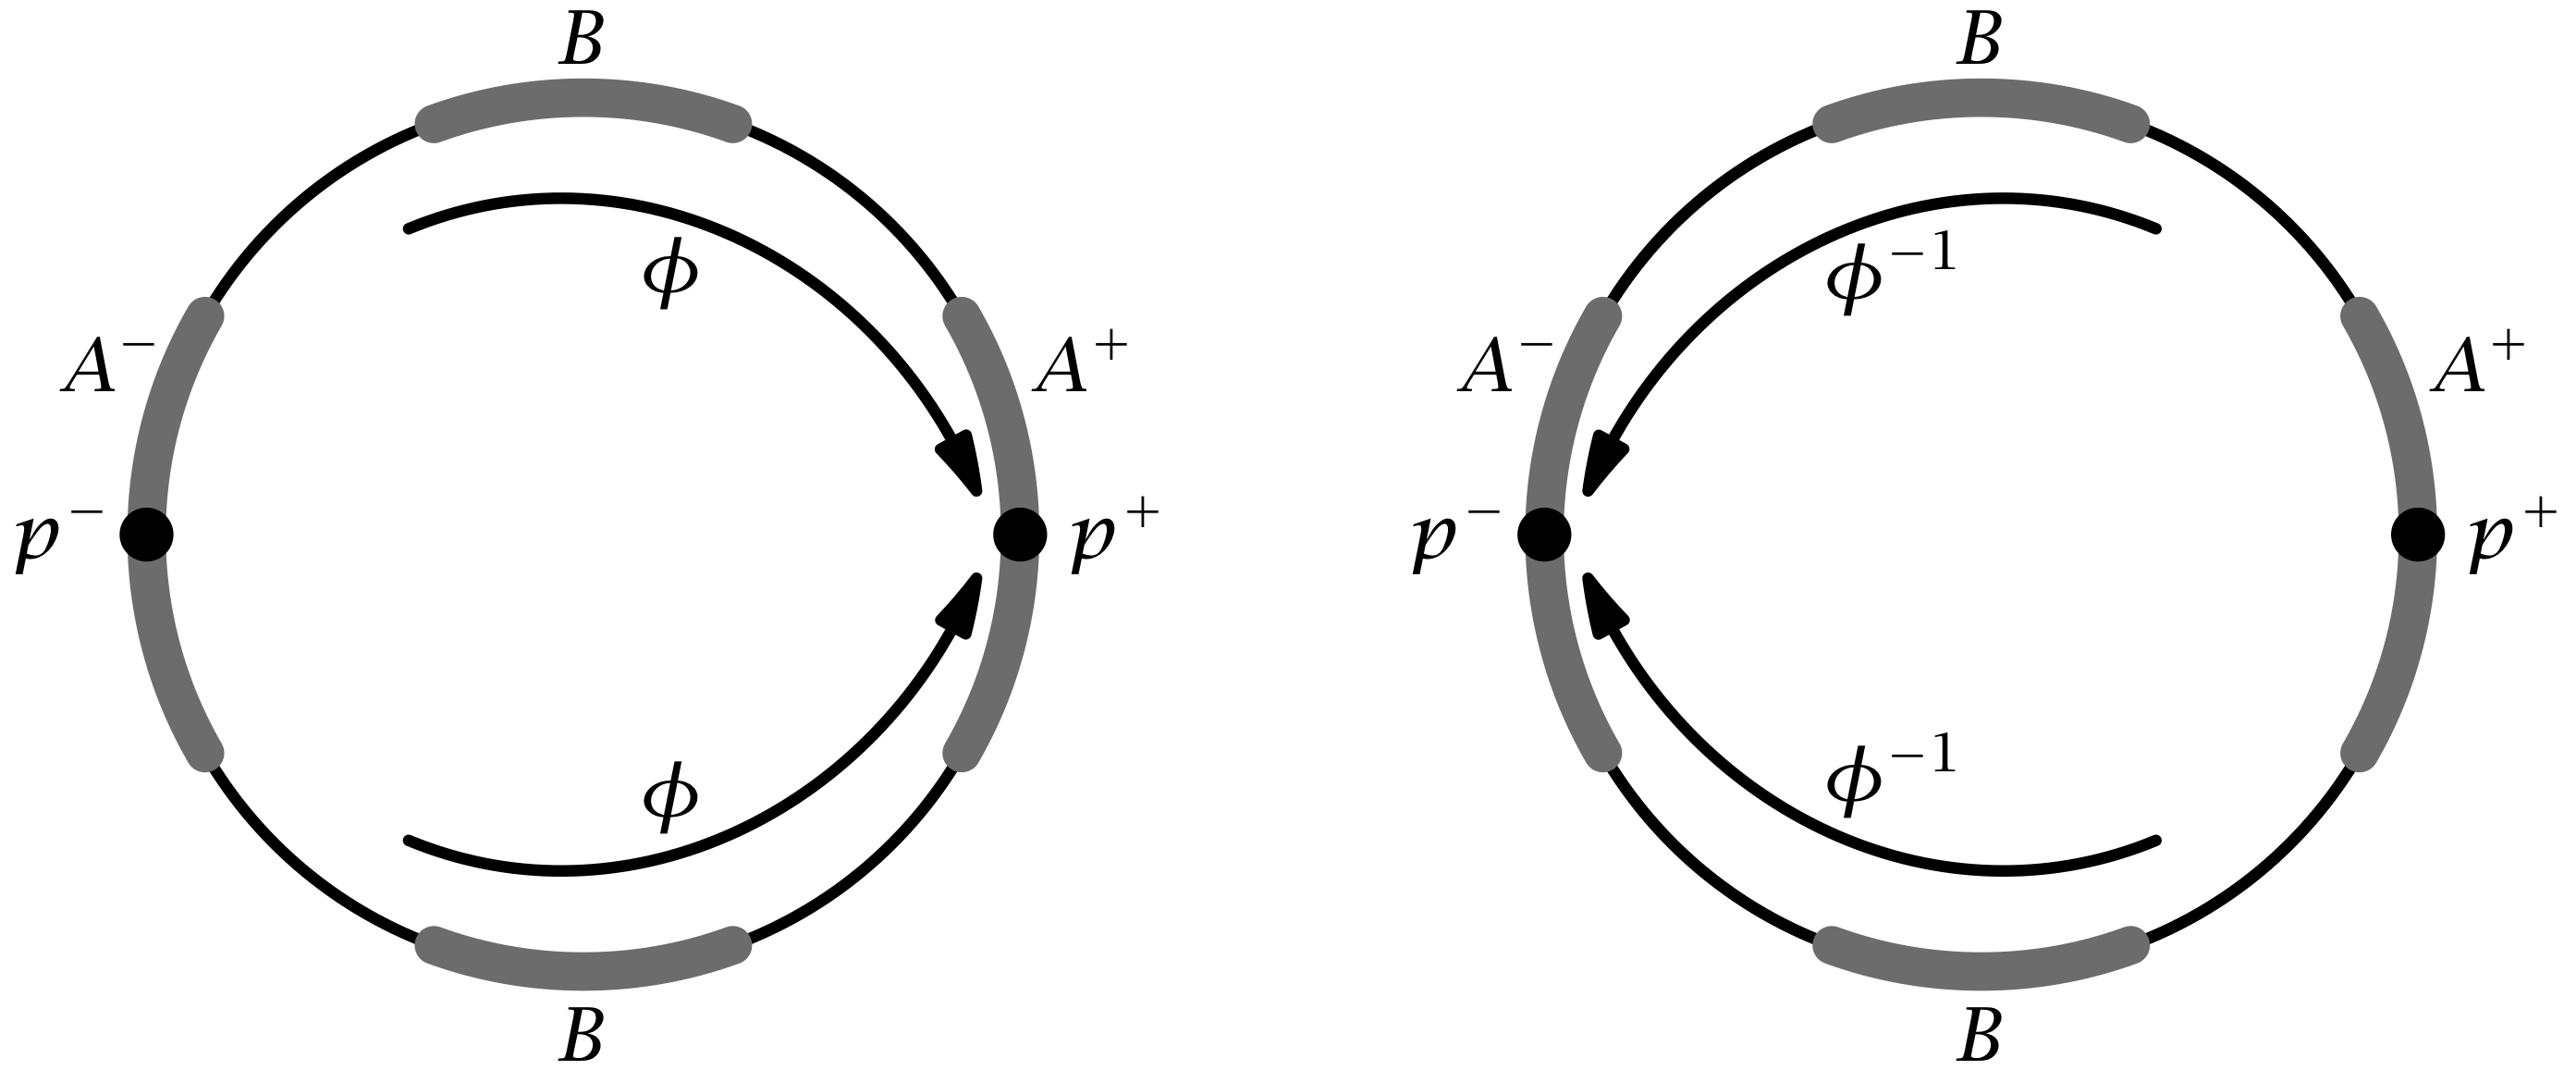
\includegraphics{PDF/Acontracting.jpg}
 \caption{A typical $(A^-,B,A^+)$-contracting
homeomorphism of the circle.} \label{Acontracting}
 \end{figure}
%texpreamble
%(" \usepackage[LY1]{fontenc}
% \usepackage[expert, LY1, mylucidascale]{mylucidabr} % I adjusted the scaling
% \usepackage{amsmath}
% \everymath{\displaystyle}
% ");
%defaultpen(  fontcommand("\normalfont") + fontsize(10) ); 
%
%from graph access *;
%
%unitsize(2cm);
%
%real r = 1, b = 3.2;
%
%currentpen=linewidth(1.5);
%
%draw( circle( (b,0) , r) );
%
%for (int i = 0; i <=1; ++i){
%	draw( circle( (i*b,0) , r) );
%
%	draw( arc( (i*b,0), r, 150, 210) , linewidth(5)+gray);
%	draw( (i*b-r,0) , linewidth(7)); 
%	label("$p^-$", (i*b-r,0) , 1.5*W);
%	label( "$A^-$", (i*b-r-0.08, 0.4*r) );
%
%	draw( arc( (i*b,0), r, -30, 30) , linewidth(5)+gray);
%	draw( (i*b+r,0) , linewidth(7)); 
%	label("$p^+$", (i*b+r,0) , 2*E);
%	label( "$A^+$", (i*b+r, 0.4*r), 0.5*E );
%
%	draw( arc( (i*b,0), r, 70, 110) , linewidth(5)+gray);
%	label( "$B$", (i*b, r), 1.5*N );
%
%	draw( arc( (i*b,0), r, -70, -110) , linewidth(5)+gray);
%	label( "$B$", (i*b, -r), 1.5*S );
%	}
%
%draw( (-0.4*r, -0.7*r){ESE}..{NNE}(0.9*r, -0.1*r), EndArrow(7) );
%draw( (-0.4*r, 0.7*r){ENE}..{SSE}(0.9*r, 0.1*r), EndArrow(7) );
%label( "$\phi$", (0.2*r, -0.6*r) ); label( "$\phi$", (0.2*r, 0.6*r) );
%
%draw( (b + 0.4*r, -0.7*r){WSW}..{NNW}(b -0.9*r, -0.1*r), EndArrow(7) );
%draw( (b + 0.4*r, 0.7*r){WNW}..{SSW}(b -0.9*r, 0.1*r), EndArrow(7) );
%label( "$\phi^{-1}$", (b - 0.2*r, -0.55*r) ); label( "$\phi^{-1}$", (b - 0.2*r, 0.6*r) );

\begin{eg} \label{22contracts}
 Let 
 \noprelistbreak
 \begin{itemize}
 \item $M$ be the real projective line
$\projective(\real^2)$, 
 \item $\gamma = 
 \begin{bmatrix}
 2 & 0 \\
 0 & 1/2
 \end{bmatrix}
 \in \SL(2,\real)$,
 \item $A^-$ be any (small) neighborhood of $p^- = [0:1]$
in $\projective(\real^2)$,
 \item $A^+$ be any (small) neighborhood of $p^+ = [1:0]$
in $\projective(\real^2)$, and
 \item $B$ be any precompact, open subset of
$\projective(\real^2) \smallsetminus \{p^-,p^+\}$.
 \end{itemize}
 For any $(x,y) \in \real^2$ with $x \neq 0$, we have
  $$\text{$\gamma^n[x:y] = [2^nx:2^{-n}y] = [1:2^{-2n}y/x] \to
[1:0] = p^+$ \  as \ $n \to \infty$} , $$
 and the convergence is uniform on
compact subsets. Similarly, we have $\gamma^{-n}[x:y] \to p^-$ as
$n \to \infty$. Hence, for sufficiently large~$n$, the
homeomorphism $\gamma^n$ is $(A^-,B,A^+)$-contracting
on $\projective(\real^2)$.
 \end{eg}

More generally, if $\gamma$~is any nontrivial, hyperbolic
element of $\SL(2,\real)$, then $\gamma^n$ is
$(A^-,B,A^+)$-contracting on $\projective(\real^2)$, for
some appropriate choice of $A^-$, $B$, and~$A^+$
\csee{hypercontracts}.

The following is easy to prove by induction on~$n$.

\begin{lem} \label{TitsPhi(A)}
 If $\phi$ is $(A^-,B,A^+)$-contracting, then
 \begin{enumerate}
 \item \label{TitsPhi(A)-A+}
 $\phi^n(B) \subseteq A^+$ for all $n > 0$,
 \item $\phi^n(B) \subseteq A^-$ for all $n < 0$,
 \item \label{TitsPhi(A)-A}
 $\phi^n(B) \subseteq A^- \cup A^+$ for all $n \neq 0$.
 \end{enumerate}
 \end{lem}

The following lemma is the key to the proof of
\cref{TitsAlternative}.

\begin{lem}[(\thmindex{Ping-Pong Lemma}Ping-Pong Lemma)] \label{PingPong}
 Suppose 
 \begin{itemize}
 \item $\phi$ and $\psi$ are homeomorphisms of a
topological space~$M$,
 \item $A^-$, $A^+$, $B^-$, and~$B^+$ are nonempty,
pairwise-disjoint, open subsets of~$M$,
 \item $\phi$ is $(A^-,B,A^+)$-contracting, where $B = B^-
\cup B^+$, and
 \item $\psi$ is $(B^-,A,B^+)$-contracting, where $A = A^-
\cup A^+$.
 \end{itemize}
 Then $\phi$ and~$\psi$ have no nontrivial relations; so
$\langle \phi, \psi \rangle$ is free.
 \end{lem}

\begin{proof}
 Consider a word of the form $w = \phi^{m_1}
\psi^{n_1} \ldots \phi^{m_k} \psi^{n_k}$, with each $m_j$
and~$n_j$ nonzero. We wish to show $w \neq e$.

From \fullcref{TitsPhi(A)}{A}, we have
 $$ \mbox{$\phi^{m_j}(B) \subseteq A$\qquad
 and\qquad
 $\psi^{n_j}(A) \subseteq B$,\qquad
 for $j = 1,2,\ldots,k$.} $$

Therefore
 \begin{align*}
 \psi^{n_k}(A) &\subseteq B, \\
 \phi^{m_k} \psi^{n_k}(A) &\subseteq A, \\
 \psi^{n_{k-1}} \phi^{m_k} \psi^{n_k}(A) &\subseteq B, \\
 \phi^{m_{k-1}} \psi^{n_{k-1}} \phi^{m_k} \psi^{n_k}(A)
&\subseteq A, 
 \end{align*}
 and so on: points bounce back and forth between~$A$
and~$B$. (Hence, the name of the \lcnamecref{PingPong}.) In the
end, we see that $w(A) \subseteq A$.

 Assume, for definiteness, that $m_1 > 0$. Then, by
applying \fullref{TitsPhi(A)}{A+} in the last step, instead
of~\fullref{TitsPhi(A)}{A}, we obtain the
more precise conclusion that $w(A) \subseteq A^+$. Since $A
\not\subseteq A^+$ (recall that $A^-$~is disjoint
from~$A^+$), we conclude that $w \neq e$, as desired.
 \end{proof}

\begin{cor} \label{hyperSL2Rfree}
 If $\gamma_1$ and~$\gamma_2$ are two nontrivial hyperbolic
elements of $\SL(2,\real)$ that have no common
eigenvector, then, for sufficiently large $n \in
\integer^+$, the group $\langle (\gamma_1)^n, (\gamma_2)^n
\rangle$ is free.
 \end{cor}

\begin{proof}
 Let 
 \noprelistbreak
 \begin{itemize}
 \item $v_j$ and~$w_j$ be linearly independent eigenvectors
of~$\gamma_j$, with eigenvalues $\lambda_j$ and
$1/\lambda_j$, such that $\lambda_j > 1$,
 \item $A^+$ and~$A^-$ be small neighborhoods of $[v_1]$
and~$[w_1]$ in $\projective(\real^2)$, and
 \item $B^+$ and~$B^-$ be small neighborhoods of $[v_2]$
and~$[w_2]$ in $\projective(\real^2)$.
 \end{itemize}
 By the same argument as in \cref{22contracts}, we see
that if $n$~is sufficiently large, then
 \begin{itemize}
 \item $(\gamma_1)^n$ is $(A^-, B^- \cup B^+,
A^+)$-contracting, and
 \item $(\gamma_2)^n$ is $(B^-, A^- \cup A^+,
B^+)$-contracting
 \end{itemize}
 \csee{hypercontracts}. Therefore, the Ping-Pong Lemma
\pref{PingPong} implies that $\langle (\gamma_1)^n,
(\gamma_2)^n \rangle$ is free.
 \end{proof}

We can now give a direct proof of \cref{FreeInGamma},
in the special case where $G = \SL(2,\real)$.

\begin{cor}
 If $G = \SL(2,\real)$, then\/ $\Gamma$ contains a
nonabelian, free group.
 \end{cor}

\begin{proof}
 By passing to a subgroup of finite index, we may assume
that $\Gamma$ is torsion free \csee{torsionfree}. Hence,
$\Gamma$ has no elliptic elements. Not every element
of~$\Gamma$ is unipotent \csee{GammaHasNonUnip}, so we
conclude that some nontrivial element~$\gamma_1$
of~$\Gamma$ is hyperbolic.

Let $v$ and~$w$ be linearly independent eigenvectors
of~$\gamma_1$. The Borel Density Theorem
\pref{BDT(Zardense)} implies that there is some $\gamma
\in \Gamma$, such that $\{\gamma v , \gamma w \} \cap
(\real v \cup \real w) = \emptyset$
\csee{gammavnotinW}. Let $\gamma_2 = \gamma \gamma_1
\gamma^{-1}$, so $\gamma_2$~is a hyperbolic element
of~$\Gamma$ with eigenvectors $\gamma v$ and~$\gamma w$.

From \cref{hyperSL2Rfree}, we conclude that
$\langle (\gamma_1)^n, (\gamma_2)^n \rangle$ is a
nonabelian, free subgroup of~$\Gamma$, for some $n \in
\integer^+$.
 \end{proof}

The same ideas work in general:

\begin{proof}[Idea of direct proof of
\cref{FreeInGamma}]
 Assume $G \subseteq \SL(\ell,\real)$. Choose some
nontrivial, hyperbolic element~$\gamma_1$ of~$\Gamma$, and let $\lambda_1 \ge \lambda_2 \ge \cdots \ge
\lambda_\ell$ be its eigenvalues. We may assume, without loss of generality,
that $\lambda_1 > \lambda_2$. (If the
eigenvalue~$\lambda_1$ has multiplicity~$d$, then we may
pass to the $d^{\text{th}}$ exterior power
$\wedge^d(\real^\ell)$, to obtain a representation in which
the largest eigenvalue of~$\gamma_1$ is simple.)

Let us assume that the smallest eigenvalue~$\lambda_\ell$
is also simple; that is, $\lambda_\ell <
\lambda_{\ell-1}$. (One can show that this is a generic
condition in~$G$, so it can be achieved by
replacing~$\gamma_1$ with some other element of~$\Gamma$.)

Let $v$ be an eigenvector corresponding to the
eigenvalue~$\lambda_1$ of~$\gamma_1$, and let $w$ be an
eigenvector for the eigenvalue~$\lambda_\ell$. Assume, to
simplify the notation, that all of the eigenspaces
of~$\gamma_1$ are orthogonal to each other. Then, for any
$x \in \real^\ell \smallsetminus v^\perp$, we have
$(\gamma_1)^n[x] \to [v]$ in $\projective(\real^\ell)$, as
$n \to \infty$ \csee{SimpleEig->Contract}. Similarly, if
$x \notin w^\perp$, then $(\gamma_1)^{-n}[x] \to [w]$.

We may assume, by replacing $\real^\ell$ with a minimal
$G$-invariant subspace, that $\real^\ell$ has no nontrivial, 
proper, $G$-invariant subspaces. Then the Borel Density Theorem implies
that there exists $\gamma \in \Gamma$, such that we have
 $\{\gamma v, \gamma w\} \cap (\real v \cup \real w) =
\emptyset$.

Then, for any small neighborhoods $A^-$, $A^+$, $B^-$,
and~$B^+$ of $[v]$, $[w]$, $[\gamma v]$, and~$[\gamma w]$,
and any sufficiently large~$n$, the Ping-Pong
Lemma implies that the subgroup $\langle (\gamma_1)^n, (\gamma \gamma_1
\gamma^{-1})^n \rangle$ is free. 
 \end{proof}

\begin{rem}
 The proof of \cref{TitsAlternative} is similar, but
involves additional complications.
 \begin{enumerate}
 \item In order to replace $\real^\ell$ with an
irreducible subspace~$W$, it is necessary to have $\dim W >
1$ (otherwise, there do not exist two linearly independent
eigenvectors $v$ and~$w$). Unfortunately, the minimal
$\Lambda$-invariant subspaces may be $1$-dimensional. 
After modding these out, the minimal subspaces in the
quotient may also be $1$-dimensional, and so on. In this
case, the group~$\Lambda$ consists entirely of
upper-triangular matrices (after a change of basis), so
$\Lambda$ is solvable.
 \item The subgroup~$\Lambda$ may not have any hyperbolic
elements. Even worse, it may be the case that $1$~is the
absolute value of every eigenvalue of every element
of~$\Lambda$. (For example, $\Lambda$ may be a subgroup of
the compact group $\SO(n)$, so that every element
of~$\Lambda$ is elliptic.) In this case, the proof replaces the
usual absolute value with an appropriate $p$-adic norm.
Not all eigenvalues are roots of unity \ccf{weaklynet}, so
Algebraic Number Theory tells us that some element
of~$\Lambda$ has an eigenvalue whose $p$-adic norm is
greater than~$1$. The proof is completed by using this eigenvalue, and the
corresponding eigenvector, just as we used~$\lambda_1$ and
the corresponding eigenvector~$v$.
 \end{enumerate}
 \end{rem}

\begin{exercises}
\item \label{hypercontracts}
 In the notation of the proof of \cref{hyperSL2Rfree},
show that if $A^-$, $A^+$, $B^-$, and~$B^+$ are disjoint,
then, for all large~$n$, the homeomorphism $(\gamma_1)^n$
is $(A^-, B^- \cup B^+, A^+)$-contracting on
$\projective(\real^2)$.

\item \label{gammavnotinW}
 Assume that $G$ is irreducible in $\SL(\ell,\real)$
\csee{irredrepDefn}, and that $\Gamma$~projects densely
into the maximal compact factor of~$G$. If $F$~is a finite
subset of $\real^\ell \smallsetminus \{0\}$, and
$\mathcal{W}$~is a finite set of proper subspaces
of~$\real^\ell$, show that there exists $\gamma \in
\Gamma$, such that 
 $$ \gamma F \cap \bigcup_{W \in \mathcal{W}} W =
\emptyset .$$
 \hint{For $v \in F$ and $W \in \mathcal{W}$, the set
 $ A_{v,W} = \{\, g \in G \mid gv \in W \,\} $
 is Zariski closed, so $\bigcup_{v,W} A_{v,W}$ is Zariski
closed. Apply the Borel Density Theorem and
\cref{Conn->ZarConn}.}

\goodbreak % @@@

\item \label{SimpleEig->Contract}
 Let 
 \noprelistbreak
 \begin{itemize}
 \item $\gamma$ be a hyperbolic element of
$\SL(\ell,\real)$, 
\item  $\lambda_1 > \lambda_2
\ge \cdots \ge \lambda_\ell$ be the eigenvalues of~$\gamma$,
 \item $v$~be an eigenvector of~$\gamma$ corresponding to
the eigenvalue~$\lambda_1$, and 
 \item $W$~be the sum of the other eigenspaces. 
 \end{itemize}
 Show that if $x \in \projective(\real^\ell)
\smallsetminus [W]$, then $\gamma^n x \to [v]$ as $n \to
\infty$. Furthermore, the convergence is uniform on
compact subsets.

\item \label{PingPongABonly}
(another version of the Ping-Pong Lemma)
Suppose $A$ and~$B$ are disjoint, nonempty subsets of~$M$, such that $\phi^n(B) \subseteq A$ and $\psi^n(A) \subseteq B$, for every \emph{nonzero} integer~$n$.
Show $\langle \phi, \psi \rangle$ is free.
\hint{If every $m_j$ and~$n_j$ is nonzero, then $\phi^{m_1} \psi^{n_1} \cdots \phi^{m_k} \psi^{n_k} \phi^{m_{k+1}}(B) \subseteq A$.}

\item \label{SanovIsFree}
Let 
	$\Gamma' = \left\langle 
	\begin{Smallbmatrix} 1 & 2 \\ 0 & 1 \end{Smallbmatrix} ,
	\begin{Smallbmatrix} 1 & 0 \\ 2 & 1 \end{Smallbmatrix} \right\rangle $
be the \defit{Sanov subgroup} of $\SL(2,\integer)$.
Show that $\Gamma'$ is a free subgroup of finite index in $\SL(2,\integer)$.
\hint{\Cref{PingPongABonly} implies $\Gamma'$ is free. 
Matrices of the form $\begin{Smallbmatrix} 4k+1 & 2\ell \\ 2m & 4n+1 \end{Smallbmatrix}$ are in~$\Gamma'$.}

\item \label{SL2ZLotsFree}
Generalizing \cref{SanovIsFree}, show that every torsion-free subgroup of $\SL(2,\integer)$ is a free group.
\hint{%Many different proofs are possible, but here is one suggestion. 
Let $\bdry\fund$ be the boundary of the usual fundamental domain for the action of $\SL(2,\integer)$ on the upper half plane~$\hyperbolic^2$ \csee{FundDomSL2R}. Then $\bigcup_{\gamma \in \Gamma} \gamma \cdot \bdry\fund$ is a contractible $1$-dimensional simplicial complex; in other words, it is a tree. $\Gamma$~acts properly on this tree, so any subgroup of~$\Gamma$ that acts freely must be a free group.}

\item \label{irredinSL2xSO3}
 Show there is an irreducible lattice~$\Gamma$ in
$\SL(2,\real) \times \SO(3)$, such that $\Gamma \cap
\SL(2,\real)$ is infinite.
 \hint{There is a free group~$F$ and a homomorphism $\phi
\colon F \to \SO(3)$, such that $\phi(F)$ is dense in
$\SO(3)$.}

\end{exercises}






\section{Moore Ergodicity Theorem} \label{MooreErgBasicSect}

All mathematicians encounter situations in which they would like to prove that some function~$\varphi$ on some space~$X$ is constant. If $X = G/\Gamma$, this means that they would like to prove $\varphi $ is $G$-invariant. 

\begin{defn}
Suppose $f$ is a function on $G/\Gamma$, and $H$~is a subgroup of~$G$. We say that $f$~is \defit[invariant function@invariant function]{$H$-invariant} if $f(hx) = f(x)$ for all $h \in H$ and $x \in G/\Gamma$.
\end{defn}

The following fundamental result shows that it suffices to prove $\varphi $ is invariant under a much smaller subgroup of~$G$ (if we make the very weak assumption that $\varphi$ is measurable). 
It does not suffice to prove that $\varphi $ is invariant under a compact subgroup, because it is easy to find a non-constant, continuous function on $G/\Gamma$ that is invariant under any given compact subgroup of~$G$ (unless $G$ itself is compact) \csee{ExistKInvtFuncs}, so the following result is optimal.


\begin{thm}[(Moore Ergodicity Theorem)] \label{MooreErgThmGsimple}
Suppose
\noprelistbreak
	\begin{itemize}
	\item $G$ is connected and simple,
	\item $H$ is a closed, noncompact subgroup of~$G$,
	and
	\item $\varphi \colon G/\Gamma \to \complex$ is $H$-invariant and measurable.
	\end{itemize}
Then $\varphi$ is constant \textup(a.e.\textup).
\end{thm}


\Cref{MooreLattFromDiscreteLp} shows how to derive this theorem from the following more general result that replaces $\Gamma$ with a discrete subgroup that need not be a lattice. (This generalization will be a crucial ingredient in \cref{SLNZISLATTSlickSect}'s proof of the important fact that $\SL(n,\integer)$ is a lattice in $\SL(n,\real)$.) In this more general situation, we impose an $\LL{p}$-integrability hypothesis on~$\varphi$, in order to compensate for the fact that $G/\Lambda$ is not assumed to have finite measure \ccf{ExistInvtNotLp}.

\begin{thm} \label{MooreErgBasicThm}
Suppose
\noprelistbreak
	\begin{itemize}
	\item $G$ is connected and simple,
	\item $H$ is a closed, noncompact subgroup of~$G$,
	\item $\Lambda$ is a discrete subgroup of~$G$,
	and
	\item $\varphi$ is an $H$-invariant $\LL{p}$-function on~$G/\Lambda$ \textup(with $1 \le p < \infty$\textup).
	\end{itemize}
Then $\varphi$ is constant \textup(a.e.\textup).
\end{thm}

\begin{proof}[Idea of proof]
To illustrate the key ingredient in the proof, let us consider only the special case where 
	$G = \SL(2,\real)$
	and 
	 $H$~is the group of diagonal matrices. 
(A proof of the general case will be given in \cref{MooreErgPfSect}.) Let
	$$ a^t = \begin{Smallbmatrix} e^t & 0 \\ 0 & e^{-t} \end{Smallbmatrix} \in H
	\qquad \text{and} \qquad
	u \in \begin{Smallbmatrix} 1& 0 \\ * & 1 \end{Smallbmatrix} .$$
Note that straightforward matrix multiplication \csee{MooreErg-commutationEx} shows
	\begin{align} \label{MooreErg-commutation}
	\lim_{t \to \infty} a^t u a^{-t} = e
	. \end{align}

For $g \in G$, define $g \varphi \colon G/\Lambda \to \complex$ by $g\varphi(x) = \varphi(g^{-1} x)$.
We are assuming that $\varphi$~is $a^t$-invariant (which means $a^t \varphi = \varphi$), and the crux of the proof is the observation that we can use \pref{MooreErg-commutation} to show that $\varphi$~must also be $u$-invariant:
we have
	\begin{align*}
	 \|u \varphi - \varphi \|_p
	&= \| a^t u \varphi - a^t \varphi \|_p 
	&& \text{(\cref{TranslateHasSameIntegral})}
	\\&= \| (a^t u a^{-t}) a^t \varphi - a^t \varphi\|_p 
	&& \text{(inserting $a^{-t} a^t$)}
	\\&= \| (a^t u a^{-t}) \varphi - \varphi \|_p 
	&& \begin{pmatrix} \text{$a^t \varphi = \varphi$ because} \\  \text{$\varphi$ is $H$-invariant} \end{pmatrix}
	\\&\to \| e \varphi - \varphi \|_p \quad \text{as $t \to \infty$} 
	&& \begin{pmatrix} \text{\pref{MooreErg-commutation} and} \\ \text{\cref{GContOnLp}} \end{pmatrix}
	\\&= 0
	, \end{align*}
so $u\varphi = \varphi$ (a.e.). 

Thus, from the fact that $\varphi$~is $H$-invariant, we have shown that 
	$$ \text{$\varphi$~must also be $\left[\begin{smallmatrix} 1& 0 \\ * & 1 \end{smallmatrix}\right]$-invariant (a.e.).} $$
The same calculation, but with $t \to -\infty$, shows that 
	$$ \text{$\varphi$ must also be $\left[\begin{smallmatrix} 1& * \\ 0 & 1 \end{smallmatrix}\right]$-invariant (a.e.).} $$
Since $\begin{Smallbmatrix} 1& 0 \\ * & 1 \end{Smallbmatrix}$ and $\begin{Smallbmatrix} 1& * \\ 0 & 1 \end{Smallbmatrix}$ generate $\SL(2,\real) = G$ \csee{ElemsGenSL2R}, we conclude that $\varphi$~is $G$-invariant (a.e.). Since $G$ is transitive on $G/\Lambda$, this implies that $\varphi$ is constant (a.e.) \csee{InvtOnTrans}.
\end{proof}

%See \cref{ErgodicChap} for more discussion of results of this type.




\begin{exercises}

\item \label{ExistKInvtFuncs}
Show that if $K$ is any compact subgroup of~$G$, and $G$ is not compact, then there is a continuous, $K$-invariant function on $G/\Gamma$ that is not constant.
%\hint{One possibility is to fix a point $p \in G/\Gamma$, and let $f(x)$ be the distance from $x$ to the $K$-orbit of~$p$.}

\item \label{ExistInvtNotLp}
Show there is a counterexample to \cref{MooreErgBasicThm} if we remove the assumption that the measurable function~$\varphi$ is~$\LL{p}$.
\hint{It is easy to construct an counterexample by taking $\Lambda$ to be trivial (or finite).}

\item \label{MooreLattFromDiscreteLp}
Derive \cref{MooreErgThmGsimple} from \cref{MooreErgBasicThm}.
\hint{If there is a nonconstant $H$-invariant function on $G/\Gamma$, then there is one that is bounded.}

\item \label{MooreErg-commutationEx}
Verify \cref{MooreErg-commutation}.

\item \label{MooreErgBasicInvtSetEx}
Suppose
	\begin{itemize} 
	\item $G$ and $H$ are as in the Moore Ergodicity Theorem \pref{MooreErgThmGsimple},
	and
	\item $X$ is an $H$-invariant, measurable subset of $G/\Gamma$.
	\end{itemize}
Show that either $X$ has measure~$0$, or the complement of~$X$ has measure~$0$.
%% \hint{The characteristic function of~$X$ is $H$-invariant.}
%\item Where does your proof use the assumption that $\Gamma$ is a lattice, rather than an arbitrary discrete subgroup?
%%\item Show there is a counterexample if we omit the assumption  that $\Lambda$ is a lattice.

\item \label{ElemsGenSL2R}
Show $\SL(2,\real)$ is generated by the subgroups
$\left\{\begin{Smallbmatrix} 1& 0 \\ * & 1 \end{Smallbmatrix}\right\}$ and $\left\{\begin{Smallbmatrix} 1& * \\ 0 & 1 \end{Smallbmatrix}\right\}$.
\hint{If a matrix can be reduced to the identity matrix by a sequence of elementary row operations, then it is a product of elementary matrices.}

\item \label{InvtOnTrans}
Suppose $\varphi$ is a measurable function on $G/\Lambda$, and for each $g \in G$, we have $\varphi(gx) = \varphi(x)$ for a.e.\ $x \in G/\Lambda$. Show $\varphi$ is constant (a.e.).
\hint{Use Fubini's Theorem to reverse the quantifiers.}

\item Suppose $G$ and $H$ are as in the Moore Ergodicity Theorem \pref{MooreErgThmGsimple}.
Show that $Hx$ is dense in $G/\Gamma$, for a.e.\ $x \in G/\Gamma$.
\hint{Use \cref{MooreErgBasicInvtSetEx}. For any open subset~$\open$ of $G/\Gamma$, the set $H\open$ is measurable (why?) and $H$-invariant.}

\item Assume $G$ is simple, and let $H$ be a subgroup of~$G$ (not necessarily closed). Show that every (real-valued) $H$-invariant measurable function on $G/\Gamma$ is constant (a.e.) if and only if the closure of $H$ is not compact.

\item \label{TranslateHasSameIntegral}
Show that if $\Lambda$ is a discrete subgroup of~$G$, and $\mu$ is a $G$-invariant measure on $G/\Lambda$, then $\int_X g\varphi \, d\mu = \int_X \varphi \, d\mu$, for every $g \in G$ and measurable $\varphi \colon G/\Lambda \to \complex$.
\hint{Apply a change of variables, and use the fact that $g_*\mu = \mu$ (since $\mu$ is $G$-invariant).}

\item \label{GContOnLp}
Show that $G$ acts continuously on $\LL{p}(G/\Lambda)$ if $1 \le p < \infty$. More precisely, show that if $\Lambda$ is a discrete subgroup of~$G$, and we define $\alpha \colon G \times \LL{p}(G/\Lambda) \to \LL{p}(G/\Lambda)$ by $\alpha(g,\varphi) = g\varphi$, then $\alpha$ is continuous.
\hint{To show $\alpha$ is continuous in~$g$, use \thmindex{Lusin's}{Lusin's Theorem} \pref{LusinsThm} to approximate~$\varphi$ by a uniformly continuous function. Then use \cref{TranslateHasSameIntegral} (and the Triangle Inequality) to complete the proof.}

\end{exercises}







\begin{notes}

Raghunathan's book \cite{RaghunathanBook} is the standard
reference for the basic properties of lattices. It contains
almost all of the material in this chapter, except the Tits
Alternative (\cref{TitsAlternativeSect}) and the Moore Ergodicity Theorem (\cref{MooreErgBasicSect}).

%Isogenies are discussed in texts, such as
%\cite{Borel-AlgicGrps}, on algebraic groups and in the book
%of Platonov and Rapinchuk \cite{PlatonovRapinchukBook}.
 
\Cref{GodementConverse} (the existence of unipotent elements in noncompact lattices) was proved by Kazhdan and Margulis \cite{KazhdanMargulis-PfSelberg}. Expositions can be found in \cite{Borel-KazhdanMargulisBourbaki} and \cite[Cor.~11.13, p.~180]{RaghunathanBook}. 

The Borel Density Theorem \pref{BDT} was proved by
Borel~\cite{Borel-BDT}. It appears in
\cite[Thm.~2.4.4, p.~93]{MargulisBook}, \cite[Thm.~5.5, p.~79]{RaghunathanBook}, and
\cite[Thm.~3.2.5, pp.~41--42]{ZimmerBook}. Several authors have published
generalizations or alternative proofs
(for example, \cite{Dani-BDT, Furstenberg-BDT,
Wigner-BDT}).
%\cite{CowlingSteger-BDT, IozziNevo-BDT, Shalom-BDT, Stuck-BDT}

Our presentation of \cref{FundDom->fg,FundDom->FinPres} is based on
\cite[pp.~195--199]{PlatonovRapinchukBook}. A proof of
\cref{LocConn->FinPres} can also be found there.
A proof of \cref{GammaFinPres} for the case where
$\Gamma$ is arithmetic can be found in
\cite{Borel-IntroGrpArith} or \cite[Thm.~4.2,
p.~195]{PlatonovRapinchukBook}. For the case where $\Qrank
\Gamma = 1$, see \cite{GarlandRaghunathan} or
\cite[Cor.~13.20, p.~210]{RaghunathanBook}.

Borel and Serre \cite[\S11.1]{BorelSerre-corners} proved $\Gamma$ is of type~$F_n$ \csee{typeFn}.
%This also follows from the theorem of Raghunathan \cite{Raghunathan-quotients} that $\Gamma \backslash G / K$ is homeomorphic to the interior of a compact manifold with boundary.
(We remark that there is no harm in assuming $\Gamma$ is torsion free, since being of type~$F_n$ is invariant under passage to finite-index subgroups \cite[Cor.~7.2.4, p.~170]{Geoghegan-TopMethGrpThy}.)

\Cref{torsionfree}
is proved in \cite[Thm.~6.11, p.~93]{RaghunathanBook} and
\cite[Cor.~17.7, p.~119]{Borel-IntroGrpArith}, in stronger forms that establish \cref{SelbergRems}(\ref{SelbergRems-net},\ref{SelbergRems-F}).
Our alternate proof of
\cref{torsionfree} is excerpted from the elementary
proof in \cite{Alperin-SelbergLemma}.

\Cref{NoTorsionFreeSubrgpWarn} is due to P.\,Deligne \cite{Deligne-torsion}.
See also \cite{Raghunathan-torsion}.

For an introduction to the Congruence Subgroup Property, see \cite[Chap.~6]{Humphreys-ArithmeticGroups} or \cite{Sury-CSPBook}.

The Tits Alternative \pref{TitsAlternative} was proved by
Tits \cite{Tits-TitsAlt}. A nice introduction (and a proof
of some special cases) can be found in
\cite{delaHarpe-TitsAlt}.

See \cref{ErgodicitySect} for more on the Moore Ergodicity Theorem \pref{MooreErgThmGsimple} and related results.

\end{notes}


\begin{references}{99}

\bibitem{Alperin-SelbergLemma}
 R.\,C.\,Alperin:
 An elementary account of Selberg's Lemma,
 \emph{L'Enseign. Math.} 33 (1987) 269--273.
\MR{0925989},
\maynewline
\url{http://dx.doi.org/10.5169/seals-87896}

\bibitem{Borel-BDT}
 A.\,Borel:
 Density properties for certain subgroups of semi-simple
groups without compact components,
 \emph{Ann. Math.} 72 (1960) 179--188.
\MR{0123639},
\maynewline
\url{http://dx.doi.org/10.2307/1970150}

\bibitem{Borel-KazhdanMargulisBourbaki}
A.\,Borel:
Sous-groupes discrets de groups semi-simples (d'apr\`es D.\,A.\,Kajdan et G.\,A.\,Margoulis),
\emph{S\'eminaire Bourbaki} 1968/1969, % (Juin 1969), 
no.~358.
\emph{Springer Lecture Notes in Math.} 175 (1971) 199--215.
\MR{3077127},
\maynewline
\url{http://www.numdam.org/item?id=SB_1968-1969__11__199_0}
%\Zbl{0225.22017}

\bibitem{Borel-IntroGrpArith}
A.\,Borel:
\emph{Introduction aux Groupes Arithm\'etiques}.
%Publications de l'Institut de MathŽmatique de l'UniversitŽe de Strasbourg, XV. ActualitŽes Scientifiques et Industrielles, No. 1341 
Hermann, Paris, 1969.
\MR{0244260}
 
\bibitem{BorelSerre-corners}
A.\,Borel and J.--P.\,Serre:
Corners and arithmetic groups,
%Avec un appendice: Arrondissement des variŽtŽs ˆ coins, par A. Douady et L. HŽrault.
\emph{Comment. Math. Helv.} 48 (1973), 436--491. 
 \MR{0387495},
 \maynewline
 \url{http://dx.doi.org/10.5169/seals-37166}
 
% \bibitem{CowlingSteger-BDT}
% M.\,Cowling and T.\,Steger:
% The irreducibility of restrictions of unitary representations to
%lattices.  
% \emphit{J. Reine Angew. Math. } 420  (1991), 85--98.
% \MRR{MR1124567}{(93e:22019)}

\bibitem{Dani-BDT}
 S.\,G.\,Dani: 
 On ergodic quasi-invariant measures of group
automorphism,
 \emph{Israel J. Math.} 43 (1982) 62--74.
 \MR{0728879},
 \url{http://dx.doi.org/10.1007/BF02761685}
 
 \bibitem{delaHarpe-TitsAlt}
 P.\,de\,la\,Harpe:
 Free groups in linear groups,
 \emph{L'Enseign. Math.} 29 (1983) 129--144.
\MR{0702736},
\maynewline
\url{http://dx.doi.org/10.5169/seals-52975}

 \bibitem{Deligne-torsion}
  P.\,Deligne:
   Extensions centrales non r\'esiduellement finies de groupes arithm\'etiques,
   \emph{C. R. Acad. Sci. Paris Ser.~A}  287  (1978), no. 4, 203--208.
  \MR{0507760} % no URL available @@@

\bibitem{Furstenberg-BDT}
 H.\,Furstenberg:
 A note on Borel's Density Theorem,
 \emph{Proc. Amer. Math. Soc.} 55 (1976) 209--212.
 \MR{0422497},
 \maynewline
 \url{http://dx.doi.org/10.1090/S0002-9939-1976-0422497-X}

\bibitem{GarlandRaghunathan}
 H.\,Garland and M.\,S.\,Raghunathan:
 Fundamental domains for lattices in ($\real$-)rank~1
semisimple Lie groups,
 \emph{Ann. Math.} 92 (1970) 279--326.
 \MR{0267041},
 \url{http://dx.doi.org/10.2307/1970838}

\bibitem{Geoghegan-TopMethGrpThy}
R.\,Geoghegan:
\emph{Topological Methods in Group Theory.}
% Graduate Texts in Mathematics, 243. 
Springer, New York, 2008.
ISBN 978-0-387-74611-1,
\MR{2365352}
 
\bibitem{Humphreys-ArithmeticGroups}
 J.\,E.\,Humphreys:
 \emph{Arithmetic Groups.}
% Lecture Notes in Mathematics \#789. 
 Springer, Berlin, 1980. 
 ISBN 3-540-09972-7,
 \MR{0584623}
 
%\bibitem{IozziNevo-BDT}
% A.\,Iozzi and A.\,Nevo:
% Algebraic hulls and the F\o lner property.  
% \emphit{Geom. Funct. Anal.} 6  (1996),  no.~4, 666--688.
% \MRR{MR1406668}{97j:22011}

\bibitem{KazhdanMargulis-PfSelberg}
D.\,Ka\v zdan and G.\,A.\,Margulis:
A proof of Selberg's hypothesis,
\emph{Math. USSR--Sbornik}  4 (1968), no.~1, 147--152.
(Translated from
\emph{Mat. Sb. (N.S.)} 75 (117) (1968) 163--168.
\MR{0223487},
\url{http://dx.doi.org/10.1070/SM1968v004n01ABEH002782}

\bibitem{MargulisBook}
 G.\,A.\,Margulis:
 \emph{Discrete Subgroups of Semisimple Lie Groups.}
 Springer, {Berlin Heidelberg New York}, 1991.
 ISBN 3-540-12179-X,
\MR{1090825}

\bibitem{PlatonovRapinchukBook}
 V.\,Platonov and A.\,Rapinchuk: 
 \emph{Algebraic Groups and Number Theory.}
 Academic Press, Boston, 1994.
 ISBN 0-12-558180-7,
 \MR{1278263}

\bibitem{RaghunathanBook}
 M.\,S.\,Raghunathan: 
 \emph{Discrete Subgroups of Lie Groups.}
 Springer, {New York}, 1972.
 ISBN 0-387-05749-8,
\MR{0507234}
 
 \bibitem{Raghunathan-torsion}
 M.\,S.\,Raghunathan: 
 Torsion in cocompact lattices in coverings of $\mathrm{Spin}(2,n)$, 
 \emph{Math. Ann.} 266 (1984), no.~4, 403--419.
 Correction \emph{Math. Ann.} 303 (1995), no.~3, 575--578.
 \MR{0735524}, \MR{1355004},
 \maynewline
  \url{http://resolver.sub.uni-goettingen.de/purl?GDZPPN002324733}, \ 
 \maynewline
\url{http://eudml.org/doc/251794}
%\url{http://www.digizeitschriften.de/dms/resolveppn/?PPN=GDZPPN002341255}

%\bibitem{Shalom-BDT}
% Y.\,Shalom:
% Invariant measures for algebraic actions, Zariski dense subgroups and
%Kazhdan's property (T).
%  \emphit{Trans. Amer. Math. Soc.}  351  (1999),  no.~8, 3387--3412.
% \MRR{MR1615966}{(99m:22008)}

%\bibitem{Stuck-BDT}
% G.\,Stuck:
% A topological analogue of the Borel density theorem.  
% \emphit{Topology}  34 (1995),  no.~1, 231--241.
% \MRR{MR1308498}{(95k:22015)}

\bibitem{Sury-CSPBook}
B.\,Sury:
\emph{The Congruence Subgroup Problem}. 
 %An elementary approach aimed at applications. Texts and Readings in Mathematics, 24. 
 Hindustan Book Agency, New Delhi, 2003.
 ISBN 81-85931-38-0,
\MR{1978430}

\bibitem{Tits-TitsAlt}
 J.\,Tits:
 Free subgroups in linear groups,
 \emph{J.~Algebra} 20 (1972) 250--270.
\MR{0286898},
\maynewline
\url{http://dx.doi.org/10.1016/0021-8693(72)90058-0}

\bibitem{Wigner-BDT}
 D.\,Wigner:
 Un th\'eor\`eme de densit\'e analytique pour les groupes
semisimples,
 \emph{Comment. Math. Helvetici} 62 (1987) 390--416.
 \MR{0910168},
 \url{http://dx.doi.org/10.5169/seals-47353}

\bibitem{ZimmerBook}
 R.\,J.\,Zimmer:
 \emph{Ergodic Theory and Semisimple Groups}.
 Birkh\"auser, Boston, 1984.
 ISBN 3-7643-3184-4,
 \MR{0776417}

 \end{references}

